\pdfoutput=1
%% Author: PGL  Porta Mana
%% Created: 2015-05-01T20:53:34+0200
%% Last-Updated: 2019-11-26T14:07:21+0100
%%%%%%%%%%%%%%%%%%%%%%%%%%%%%%%%%%%%%%%%%%%%%%%%%%%%%%%%%%%%%%%%%%%%%%%%%%%%
\newif\ifarxiv
\arxivfalse
\ifarxiv\pdfmapfile{+classico.map}\fi
\newif\ifafour
\afourfalse% true = A4, false = A5
\newif\iftypodisclaim % typographical disclaim on the side
\typodisclaimtrue
\newcommand*{\memfontfamily}{zplx}
\newcommand*{\memfontpack}{newpxtext}
\documentclass[\ifafour a4paper,12pt,\else a5paper,10pt,\fi%extrafontsizes,%
onecolumn,oneside,article,%french,italian,german,swedish,latin,
british%
]{memoir}
\newcommand*{\updated}{\today}
\newcommand*{\firstdraft}{4 November 2015}
\newcommand*{\firstpublished}{***}
\newcommand*{\propertitle}{Maximum-entropy distributions for a 
  neuronal population\\ from subpopulation data {\large\color{myred}[draft]}%\\{\large ***}%
}
\newcommand*{\pdftitle}{\propertitle}
\newcommand*{\headtitle}{Maximum-entropy from sample data}
\newcommand*{\pdfauthor}{P.G.L.  Porta Mana, Y. Roudi, V. Rostami, E. Torre}
\newcommand*{\headauthor}{Porta Mana \etal}
\newcommand*{\reporthead}{}% Report number

%%%%%%%%%%%%%%%%%%%%%%%%%%%%%%%%%%%%%%%%%%%%%%%%%%%%%%%%%%%%%%%%%%%%%%%%%%%%
%%% Calls to packages (uncomment as needed)
%%%%%%%%%%%%%%%%%%%%%%%%%%%%%%%%%%%%%%%%%%%%%%%%%%%%%%%%%%%%%%%%%%%%%%%%%%%%

%\usepackage{pifont}

%\usepackage{fontawesome}

\usepackage[T1]{fontenc} 
\input{glyphtounicode} \pdfgentounicode=1

\usepackage[utf8]{inputenx}

%\usepackage{newunicodechar}
% \newunicodechar{Ĕ}{\u{E}}
% \newunicodechar{ĕ}{\u{e}}
% \newunicodechar{Ĭ}{\u{I}}
% \newunicodechar{ĭ}{\u{\i}}
% \newunicodechar{Ŏ}{\u{O}}
% \newunicodechar{ŏ}{\u{o}}
% \newunicodechar{Ŭ}{\u{U}}
% \newunicodechar{ŭ}{\u{u}}
% \newunicodechar{Ā}{\=A}
% \newunicodechar{ā}{\=a}
% \newunicodechar{Ē}{\=E}
% \newunicodechar{ē}{\=e}
% \newunicodechar{Ī}{\=I}
% \newunicodechar{ī}{\={\i}}
% \newunicodechar{Ō}{\=O}
% \newunicodechar{ō}{\=o}
% \newunicodechar{Ū}{\=U}
% \newunicodechar{ū}{\=u}
% \newunicodechar{Ȳ}{\=Y}
% \newunicodechar{ȳ}{\=y}

\newcommand*{\bmmax}{0} % reduce number of bold fonts, before font packages
\newcommand*{\hmmax}{0} % reduce number of heavy fonts, before font packages

\usepackage{textcomp}

%\usepackage[normalem]{ulem}% package for underlining
% \makeatletter
% \def\ssout{\bgroup \ULdepth=-.35ex%\UL@setULdepth
%  \markoverwith{\lower\ULdepth\hbox
%    {\kern-.03em\vbox{\hrule width.2em\kern1.2\p@\hrule}\kern-.03em}}%
%  \ULon}
% \makeatother

\usepackage{amsmath}

\usepackage{mathtools}
\addtolength{\jot}{\jot} % increase spacing in multiline formulae
\setlength{\multlinegap}{0pt}

%\usepackage{empheq}% automatically calls amsmath and mathtools
%\newcommand*{\widefbox}[1]{\fbox{\hspace{1em}#1\hspace{1em}}}

%\usepackage{fancybox}

%\usepackage{framed}

% \usepackage[misc]{ifsym} % for dice
% \newcommand*{\diceone}{{\scriptsize\Cube{1}}}

\usepackage{amssymb}

\usepackage{amsxtra}

\usepackage[main=british,french,italian,german,swedish,latin,esperanto]{babel}\selectlanguage{british}
\newcommand*{\langfrench}{\foreignlanguage{french}}
\newcommand*{\langgerman}{\foreignlanguage{german}}
\newcommand*{\langitalian}{\foreignlanguage{italian}}
\newcommand*{\langswedish}{\foreignlanguage{swedish}}
\newcommand*{\langlatin}{\foreignlanguage{latin}}
\newcommand*{\langnohyph}{\foreignlanguage{nohyphenation}}

\usepackage[autostyle=false,autopunct=false,english=british]{csquotes}
\setquotestyle{british}

\usepackage{amsthm}
\newcommand*{\QED}{\textsc{q.e.d.}}
\renewcommand*{\qedsymbol}{\QED}
\theoremstyle{remark}
\newtheorem{note}{Note}
\newtheorem*{remark}{Note}
\newtheoremstyle{innote}{\parsep}{\parsep}{\footnotesize}{}{}{}{0pt}{}
\theoremstyle{innote}
\newtheorem*{innote}{}

\usepackage[shortlabels,inline]{enumitem}
\SetEnumitemKey{para}{itemindent=\parindent,leftmargin=0pt,listparindent=\parindent,parsep=0pt,itemsep=\topsep}
% \begin{asparaenum} = \begin{enumerate}[para]
% \begin{inparaenum} = \begin{enumerate*}
\setlist[enumerate,2]{label=\alph*.}
\setlist[enumerate]{label=\arabic*.,leftmargin=1.5\parindent}
\setlist[itemize]{leftmargin=1.5\parindent}
\setlist[description]{leftmargin=1.5\parindent}
% old alternative:
% \setlist[enumerate,2]{label=\alph*.}
% \setlist[enumerate]{leftmargin=\parindent}
% \setlist[itemize]{leftmargin=\parindent}
% \setlist[description]{leftmargin=\parindent}

\usepackage[babel,theoremfont,largesc]{newpxtext}

\usepackage[bigdelims,nosymbolsc%,smallerops % probably arXiv doesn't have it
]{newpxmath}
\linespread{1.083}%\useosf
%% smaller operators for old version of newpxmath
\makeatletter
\def\re@DeclareMathSymbol#1#2#3#4{%
    \let#1=\undefined
    \DeclareMathSymbol{#1}{#2}{#3}{#4}}
%\re@DeclareMathSymbol{\bigsqcupop}{\mathop}{largesymbols}{"46}
%\re@DeclareMathSymbol{\bigodotop}{\mathop}{largesymbols}{"4A}
\re@DeclareMathSymbol{\bigoplusop}{\mathop}{largesymbols}{"4C}
\re@DeclareMathSymbol{\bigotimesop}{\mathop}{largesymbols}{"4E}
\re@DeclareMathSymbol{\sumop}{\mathop}{largesymbols}{"50}
\re@DeclareMathSymbol{\prodop}{\mathop}{largesymbols}{"51}
\re@DeclareMathSymbol{\bigcupop}{\mathop}{largesymbols}{"53}
\re@DeclareMathSymbol{\bigcapop}{\mathop}{largesymbols}{"54}
%\re@DeclareMathSymbol{\biguplusop}{\mathop}{largesymbols}{"55}
\re@DeclareMathSymbol{\bigwedgeop}{\mathop}{largesymbols}{"56}
\re@DeclareMathSymbol{\bigveeop}{\mathop}{largesymbols}{"57}
%\re@DeclareMathSymbol{\bigcupdotop}{\mathop}{largesymbols}{"DF}
%\re@DeclareMathSymbol{\bigcapplusop}{\mathop}{largesymbolsPXA}{"00}
%\re@DeclareMathSymbol{\bigsqcupplusop}{\mathop}{largesymbolsPXA}{"02}
%\re@DeclareMathSymbol{\bigsqcapplusop}{\mathop}{largesymbolsPXA}{"04}
%\re@DeclareMathSymbol{\bigsqcapop}{\mathop}{largesymbolsPXA}{"06}
\re@DeclareMathSymbol{\bigtimesop}{\mathop}{largesymbolsPXA}{"10}
%\re@DeclareMathSymbol{\coprodop}{\mathop}{largesymbols}{"60}
%\re@DeclareMathSymbol{\varprod}{\mathop}{largesymbolsPXA}{16}
\makeatother
%%
%% With euler font cursive for Greek letters - the [1] means 100% scaling
\DeclareFontFamily{U}{egreek}{\skewchar\font'177}%
\DeclareFontShape{U}{egreek}{m}{n}{<-6>s*[1]eurm5 <6-8>s*[1]eurm7 <8->s*[1]eurm10}{}%
\DeclareFontShape{U}{egreek}{m}{it}{<->s*[1]eurmo10}{}%
\DeclareFontShape{U}{egreek}{b}{n}{<-6>s*[1]eurb5 <6-8>s*[1]eurb7 <8->s*[1]eurb10}{}%
\DeclareFontShape{U}{egreek}{b}{it}{<->s*[1]eurbo10}{}%
\DeclareSymbolFont{egreeki}{U}{egreek}{m}{it}%
\SetSymbolFont{egreeki}{bold}{U}{egreek}{b}{it}% from the amsfonts package
\DeclareSymbolFont{egreekr}{U}{egreek}{m}{n}%
\SetSymbolFont{egreekr}{bold}{U}{egreek}{b}{n}% from the amsfonts package
% Take also \sum, \prod, \coprod symbols from Euler fonts
\DeclareFontFamily{U}{egreekx}{\skewchar\font'177}
\DeclareFontShape{U}{egreekx}{m}{n}{%
       <-7.5>s*[0.9]euex7%
    <7.5-8.5>s*[0.9]euex8%
    <8.5-9.5>s*[0.9]euex9%
    <9.5->s*[0.9]euex10%
}{}
\DeclareSymbolFont{egreekx}{U}{egreekx}{m}{n}
\DeclareMathSymbol{\sumop}{\mathop}{egreekx}{"50}
\DeclareMathSymbol{\prodop}{\mathop}{egreekx}{"51}
\DeclareMathSymbol{\coprodop}{\mathop}{egreekx}{"60}
\makeatletter
\def\sum{\DOTSI\sumop\slimits@}
\def\prod{\DOTSI\prodop\slimits@}
\def\coprod{\DOTSI\coprodop\slimits@}
\makeatother
% Greek letters not usually given in LaTeX.
\DeclareMathSymbol{\varpartial}{\mathalpha}{egreeki}{"40}
\DeclareMathSymbol{\partialup}{\mathalpha}{egreekr}{"40}
\DeclareMathSymbol{\alpha}{\mathalpha}{egreeki}{"0B}
\DeclareMathSymbol{\beta}{\mathalpha}{egreeki}{"0C}
\DeclareMathSymbol{\gamma}{\mathalpha}{egreeki}{"0D}
\DeclareMathSymbol{\delta}{\mathalpha}{egreeki}{"0E}
\DeclareMathSymbol{\epsilon}{\mathalpha}{egreeki}{"0F}
\DeclareMathSymbol{\zeta}{\mathalpha}{egreeki}{"10}
\DeclareMathSymbol{\eta}{\mathalpha}{egreeki}{"11}
\DeclareMathSymbol{\theta}{\mathalpha}{egreeki}{"12}
\DeclareMathSymbol{\iota}{\mathalpha}{egreeki}{"13}
\DeclareMathSymbol{\kappa}{\mathalpha}{egreeki}{"14}
\DeclareMathSymbol{\lambda}{\mathalpha}{egreeki}{"15}
\DeclareMathSymbol{\mu}{\mathalpha}{egreeki}{"16}
\DeclareMathSymbol{\nu}{\mathalpha}{egreeki}{"17}
\DeclareMathSymbol{\xi}{\mathalpha}{egreeki}{"18}
\DeclareMathSymbol{\omicron}{\mathalpha}{egreeki}{"6F}
\DeclareMathSymbol{\pi}{\mathalpha}{egreeki}{"19}
\DeclareMathSymbol{\rho}{\mathalpha}{egreeki}{"1A}
\DeclareMathSymbol{\sigma}{\mathalpha}{egreeki}{"1B}
 \DeclareMathSymbol{\tau}{\mathalpha}{egreeki}{"1C}
\DeclareMathSymbol{\upsilon}{\mathalpha}{egreeki}{"1D}
\DeclareMathSymbol{\phi}{\mathalpha}{egreeki}{"1E}
\DeclareMathSymbol{\chi}{\mathalpha}{egreeki}{"1F}
\DeclareMathSymbol{\psi}{\mathalpha}{egreeki}{"20}
\DeclareMathSymbol{\omega}{\mathalpha}{egreeki}{"21}
\DeclareMathSymbol{\varepsilon}{\mathalpha}{egreeki}{"22}
\DeclareMathSymbol{\vartheta}{\mathalpha}{egreeki}{"23}
\DeclareMathSymbol{\varpi}{\mathalpha}{egreeki}{"24}
\let\varrho\rho 
\let\varsigma\sigma
 \let\varkappa\kappa
\DeclareMathSymbol{\varphi}{\mathalpha}{egreeki}{"27}
%
\DeclareMathSymbol{\varAlpha}{\mathalpha}{egreeki}{"41}
\DeclareMathSymbol{\varBeta}{\mathalpha}{egreeki}{"42}
\DeclareMathSymbol{\varGamma}{\mathalpha}{egreeki}{"00}
\DeclareMathSymbol{\varDelta}{\mathalpha}{egreeki}{"01}
\DeclareMathSymbol{\varEpsilon}{\mathalpha}{egreeki}{"45}
\DeclareMathSymbol{\varZeta}{\mathalpha}{egreeki}{"5A}
\DeclareMathSymbol{\varEta}{\mathalpha}{egreeki}{"48}
\DeclareMathSymbol{\varTheta}{\mathalpha}{egreeki}{"02}
 \DeclareMathSymbol{\varIota}{\mathalpha}{egreeki}{"49}
\DeclareMathSymbol{\varKappa}{\mathalpha}{egreeki}{"4B}
\DeclareMathSymbol{\varLambda}{\mathalpha}{egreeki}{"03}
\DeclareMathSymbol{\varMu}{\mathalpha}{egreeki}{"4D}
\DeclareMathSymbol{\varNu}{\mathalpha}{egreeki}{"4E}
\DeclareMathSymbol{\varXi}{\mathalpha}{egreeki}{"04}
\DeclareMathSymbol{\varOmicron}{\mathalpha}{egreeki}{"4F}
\DeclareMathSymbol{\varPi}{\mathalpha}{egreeki}{"05}
\DeclareMathSymbol{\varRho}{\mathalpha}{egreeki}{"50}
\DeclareMathSymbol{\varSigma}{\mathalpha}{egreeki}{"06}
\DeclareMathSymbol{\varTau}{\mathalpha}{egreeki}{"54}
\DeclareMathSymbol{\varUpsilon}{\mathalpha}{egreeki}{"07}
\DeclareMathSymbol{\varPhi}{\mathalpha}{egreeki}{"08}
\DeclareMathSymbol{\varChi}{\mathalpha}{egreeki}{"58}
\DeclareMathSymbol{\varPsi}{\mathalpha}{egreeki}{"09}
\DeclareMathSymbol{\varOmega}{\mathalpha}{egreeki}{"0A} 
%
\DeclareMathSymbol{\Alpha}{\mathalpha}{egreekr}{"41}
\DeclareMathSymbol{\Beta}{\mathalpha}{egreekr}{"42}
\DeclareMathSymbol{\Gamma}{\mathalpha}{egreekr}{"00}
\DeclareMathSymbol{\Delta}{\mathalpha}{egreekr}{"01}
\DeclareMathSymbol{\Epsilon}{\mathalpha}{egreekr}{"45}
\DeclareMathSymbol{\Zeta}{\mathalpha}{egreekr}{"5A}
\DeclareMathSymbol{\Eta}{\mathalpha}{egreekr}{"48}
\DeclareMathSymbol{\Theta}{\mathalpha}{egreekr}{"02}
\DeclareMathSymbol{\Iota}{\mathalpha}{egreekr}{"49}
\DeclareMathSymbol{\Kappa}{\mathalpha}{egreekr}{"4B}
\DeclareMathSymbol{\Lambda}{\mathalpha}{egreekr}{"03}
\DeclareMathSymbol{\Mu}{\mathalpha}{egreekr}{"4D}
\DeclareMathSymbol{\Nu}{\mathalpha}{egreekr}{"4E}
\DeclareMathSymbol{\Xi}{\mathalpha}{egreekr}{"04}
\DeclareMathSymbol{\Omicron}{\mathalpha}{egreekr}{"4F}
\DeclareMathSymbol{\Pi}{\mathalpha}{egreekr}{"05}
\DeclareMathSymbol{\Rho}{\mathalpha}{egreekr}{"50}
\DeclareMathSymbol{\Sigma}{\mathalpha}{egreekr}{"06}
\DeclareMathSymbol{\Tau}{\mathalpha}{egreekr}{"54}
\DeclareMathSymbol{\Upsilon}{\mathalpha}{egreekr}{"07}
\DeclareMathSymbol{\Phi}{\mathalpha}{egreekr}{"08}
\DeclareMathSymbol{\Chi}{\mathalpha}{egreekr}{"58}
\DeclareMathSymbol{\Psi}{\mathalpha}{egreekr}{"09}
\DeclareMathSymbol{\Omega}{\mathalpha}{egreekr}{"0A}
%
\DeclareMathSymbol{\alphaup}{\mathalpha}{egreekr}{"0B}
\DeclareMathSymbol{\betaup}{\mathalpha}{egreekr}{"0C}
\DeclareMathSymbol{\gammaup}{\mathalpha}{egreekr}{"0D}
 \DeclareMathSymbol{\deltaup}{\mathalpha}{egreekr}{"0E}
\DeclareMathSymbol{\epsilonup}{\mathalpha}{egreekr}{"0F}
\DeclareMathSymbol{\zetaup}{\mathalpha}{egreekr}{"10}
\DeclareMathSymbol{\etaup}{\mathalpha}{egreekr}{"11}
\DeclareMathSymbol{\thetaup}{\mathalpha}{egreekr}{"12}
\DeclareMathSymbol{\iotaup}{\mathalpha}{egreekr}{"13}
\DeclareMathSymbol{\kappaup}{\mathalpha}{egreekr}{"14}
\DeclareMathSymbol{\lambdaup}{\mathalpha}{egreekr}{"15}
\DeclareMathSymbol{\muup}{\mathalpha}{egreekr}{"16}
\DeclareMathSymbol{\nuup}{\mathalpha}{egreekr}{"17}
\DeclareMathSymbol{\xiup}{\mathalpha}{egreekr}{"18}
\DeclareMathSymbol{\omicronup}{\mathalpha}{egreekr}{"6F}
  \DeclareMathSymbol{\piup}{\mathalpha}{egreekr}{"19}
\DeclareMathSymbol{\rhoup}{\mathalpha}{egreekr}{"1A}
\DeclareMathSymbol{\sigmaup}{\mathalpha}{egreekr}{"1B}
\DeclareMathSymbol{\tauup}{\mathalpha}{egreekr}{"1C}
\DeclareMathSymbol{\upsilonup}{\mathalpha}{egreekr}{"1D}
\DeclareMathSymbol{\phiup}{\mathalpha}{egreekr}{"1E}
\DeclareMathSymbol{\chiup}{\mathalpha}{egreekr}{"1F}
\DeclareMathSymbol{\psiup}{\mathalpha}{egreekr}{"20}
\DeclareMathSymbol{\omegaup}{\mathalpha}{egreekr}{"21}
\DeclareMathSymbol{\varepsilonup}{\mathalpha}{egreekr}{"22}
\DeclareMathSymbol{\varthetaup}{\mathalpha}{egreekr}{"23}
\DeclareMathSymbol{\varpiup}{\mathalpha}{egreekr}{"24}
\let\varrhoup\rhoup 
\let\varsigmaup\sigmaup
\let\varkappaup\kappaup
\DeclareMathSymbol{\varphiup}{\mathalpha}{egreekr}{"27}
% Greek letters not usually given in LaTeX.

%\usepackage%[scaled=0.9]%
%{classico}%  Optima as sans-serif font
\renewcommand\sfdefault{uop}
\DeclareMathAlphabet{\mathsf}  {T1}{\sfdefault}{m}{sl}
\SetMathAlphabet{\mathsf}{bold}{T1}{\sfdefault}{b}{sl}
\newcommand*{\mathte}[1]{\textbf{\textit{\textsf{#1}}}}
% Upright sans-serif math alphabet
% \DeclareMathAlphabet{\mathsu}  {T1}{\sfdefault}{m}{n}
% \SetMathAlphabet{\mathsu}{bold}{T1}{\sfdefault}{b}{n}

% DejaVu Mono as typewriter text
\usepackage[scaled=0.84]{DejaVuSansMono}

\usepackage{mathdots}

\usepackage[usenames]{xcolor}
% Tol (2012) colour-blind-, print-, screen-friendly colours, alternative scheme; Munsell terminology
\definecolor{mypurpleblue}{RGB}{68,119,170}
\definecolor{myblue}{RGB}{102,204,238}
\definecolor{mygreen}{RGB}{34,136,51}
\definecolor{myyellow}{RGB}{204,187,68}
\definecolor{myred}{RGB}{238,102,119}
\definecolor{myredpurple}{RGB}{170,51,119}
\definecolor{mygrey}{RGB}{187,187,187}
% Tol (2012) colour-blind-, print-, screen-friendly colours; Munsell terminology
% \definecolor{lbpurple}{RGB}{51,34,136}
% \definecolor{lblue}{RGB}{136,204,238}
% \definecolor{lbgreen}{RGB}{68,170,153}
% \definecolor{lgreen}{RGB}{17,119,51}
% \definecolor{lgyellow}{RGB}{153,153,51}
% \definecolor{lyellow}{RGB}{221,204,119}
% \definecolor{lred}{RGB}{204,102,119}
% \definecolor{lpred}{RGB}{136,34,85}
% \definecolor{lrpurple}{RGB}{170,68,153}
\definecolor{lgrey}{RGB}{221,221,221}
%\newcommand*\mycolourbox[1]{%
%\colorbox{mygrey}{\hspace{1em}#1\hspace{1em}}}
\colorlet{shadecolor}{lgrey}

\usepackage{bm}

\usepackage{microtype}

\usepackage[backend=biber,mcite,%subentry,
citestyle=authoryear-comp,bibstyle=pglpm-authoryear,autopunct=false,sorting=ny,sortcites=false,natbib=false,maxcitenames=1,maxbibnames=8,minbibnames=8,giveninits=true,uniquename=false,uniquelist=false,maxalphanames=1,block=space,hyperref=true,defernumbers=false,useprefix=true,sortupper=false,language=british,parentracker=false]{biblatex}
\DeclareSortingScheme{ny}{\sort{\field{sortname}\field{author}\field{editor}}\sort{\field{year}}}
\iffalse\makeatletter%%% replace parenthesis with brackets
\newrobustcmd*{\parentexttrack}[1]{%
  \begingroup
  \blx@blxinit
  \blx@setsfcodes
  \blx@bibopenparen#1\blx@bibcloseparen
  \endgroup}
\AtEveryCite{%
  \let\parentext=\parentexttrack%
  \let\bibopenparen=\bibopenbracket%
  \let\bibcloseparen=\bibclosebracket}
\makeatother\fi
\DefineBibliographyExtras{british}{\def\finalandcomma{\addcomma}}
\renewcommand*{\finalnamedelim}{\addcomma\space}
\setcounter{biburlnumpenalty}{1}
\setcounter{biburlucpenalty}{0}
\setcounter{biburllcpenalty}{1}
\DeclareDelimFormat{multicitedelim}{\addsemicolon\space}
\DeclareDelimFormat{compcitedelim}{\addsemicolon\space}
\DeclareDelimFormat{postnotedelim}{\space}
\ifarxiv\else\addbibresource{portamanabib.bib}\fi
\renewcommand{\bibfont}{\footnotesize}
%\appto{\citesetup}{\footnotesize}% smaller font for citations
\defbibheading{bibliography}[\bibname]{\section*{#1}\addcontentsline{toc}{section}{#1}%\markboth{#1}{#1}
}
\newcommand*{\citep}{\footcites}
\newcommand*{\citey}{\parencites*}
%\renewcommand*{\cite}{\parencite}
%\newcommand*{\citeps}{\parencites}
\providecommand{\href}[2]{#2}
\providecommand{\eprint}[2]{\texttt{\href{#1}{#2}}}
\newcommand*{\amp}{\&}
% \newcommand*{\citein}[2][]{\textnormal{\textcite[#1]{#2}}%\addtocategory{extras}{#2}
% }
\newcommand*{\citein}[2][]{\textnormal{\textcite[#1]{#2}}%\addtocategory{extras}{#2}
}
\newcommand*{\citebi}[2][]{\textcite[#1]{#2}%\addtocategory{extras}{#2}
}
\newcommand*{\subtitleproc}[1]{}
\newcommand*{\chapb}{ch.}
%
% \def\arxivp{}
% \def\mparcp{}
% \def\philscip{}
% \def\biorxivp{}
% \newcommand*{\arxivsi}{\texttt{arXiv} eprints available at \url{http://arxiv.org/}.\\}
% \newcommand*{\mparcsi}{\texttt{mp\_arc} eprints available at \url{http://www.ma.utexas.edu/mp_arc/}.\\}
% \newcommand*{\philscisi}{\texttt{philsci} eprints available at \url{http://philsci-archive.pitt.edu/}.\\}
% \newcommand*{\biorxivsi}{\texttt{bioRxiv} eprints available at \url{http://biorxiv.org/}.\\}
\newcommand*{\arxiveprint}[1]{%\global\def\arxivp{\arxivsi}%\citeauthor{0arxivcite}\addtocategory{ifarchcit}{0arxivcite}%eprint
\texttt{\urlalt{https://arxiv.org/abs/#1}{arXiv:\hspace{0pt}#1}}%
%\texttt{\href{http://arxiv.org/abs/#1}{\protect\url{arXiv:#1}}}%
%\renewcommand{\arxivnote}{\texttt{arXiv} eprints available at \url{http://arxiv.org/}.}
}
\newcommand*{\mparceprint}[1]{%\global\def\mparcp{\mparcsi}%\citeauthor{0mparccite}\addtocategory{ifarchcit}{0mparccite}%eprint
\texttt{\urlalt{http://www.ma.utexas.edu/mp_arc-bin/mpa?yn=#1}{mp\_arc:\hspace{0pt}#1}}%
%\texttt{\href{http://www.ma.utexas.edu/mp_arc-bin/mpa?yn=#1}{\protect\url{mp_arc:#1}}}%
%\providecommand{\mparcnote}{\texttt{mp_arc} eprints available at \url{http://www.ma.utexas.edu/mp_arc/}.}
}
\newcommand*{\haleprint}[1]{%\global\def\arxivp{\arxivsi}%\citeauthor{0arxivcite}\addtocategory{ifarchcit}{0arxivcite}%eprint
\texttt{\urlalt{https://hal.archives-ouvertes.fr/#1}{HAL:\hspace{0pt}#1}}%
%\texttt{\href{http://arxiv.org/abs/#1}{\protect\url{arXiv:#1}}}%
%\renewcommand{\arxivnote}{\texttt{arXiv} eprints available at \url{http://arxiv.org/}.}
}
\newcommand*{\philscieprint}[1]{%\global\def\philscip{\philscisi}%\citeauthor{0philscicite}\addtocategory{ifarchcit}{0philscicite}%eprint
\texttt{\urlalt{http://philsci-archive.pitt.edu/archive/#1}{PhilSci:\hspace{0pt}#1}}%
%\texttt{\href{http://philsci-archive.pitt.edu/archive/#1}{\protect\url{PhilSci:#1}}}%
%\providecommand{\mparcnote}{\texttt{philsci} eprints available at \url{http://philsci-archive.pitt.edu/}.}
}
\newcommand*{\biorxiveprint}[1]{%\global\def\biorxivp{\biorxivsi}%\citeauthor{0arxivcite}\addtocategory{ifarchcit}{0arxivcite}%eprint
\texttt{\urlalt{https://doi.org/10.1101/#1}{bioRxiv doi:\hspace{0pt}10.1101/#1}}%
%\texttt{\href{http://arxiv.org/abs/#1}{\protect\url{arXiv:#1}}}%
%\renewcommand{\arxivnote}{\texttt{arXiv} eprints available at \url{http://arxiv.org/}.}
}
\newcommand*{\osfeprint}[1]{%
\texttt{\urlalt{https://doi.org/10.17605/osf.io/#1}{Open Science Framework doi:10.17605/osf.io/#1}}%
}

\usepackage{graphicx}

%\usepackage{wrapfig}

%\usepackage{tikz-cd}

\PassOptionsToPackage{hyphens}{url}\usepackage[hypertexnames=false]{hyperref}

\usepackage[depth=4]{bookmark}
\hypersetup{colorlinks=true,bookmarksnumbered,pdfborder={0 0 0.25},citebordercolor={0.2667 0.4667 0.6667},citecolor=mypurpleblue,linkbordercolor={0.6667 0.2 0.4667},linkcolor=myredpurple,urlbordercolor={0.1333 0.5333 0.2},urlcolor=mygreen,breaklinks=true,pdftitle={\pdftitle},pdfauthor={\pdfauthor}}
% \usepackage[vertfit=local]{breakurl}% only for arXiv
\providecommand*{\urlalt}{\href}

\usepackage[british]{datetime2}
\DTMnewdatestyle{mydate}%
{% definitions
\renewcommand*{\DTMdisplaydate}[4]{%
\number##3\ \DTMenglishmonthname{##2} ##1}%
\renewcommand*{\DTMDisplaydate}{\DTMdisplaydate}%
}
\DTMsetdatestyle{mydate}

%%%%%%%%%%%%%%%%%%%%%%%%%%%%%%%%%%%%%%%%%%%%%%%%%%%%%%%%%%%%%%%%%%%%%%%%%%%%
%%% Layout. I do not know on which kind of paper the reader will print the
%%% paper on (A4? letter? one-sided? double-sided?). So I choose A5, which
%%% provides a good layout for reading on screen and save paper if printed
%%% two pages per sheet. Average length line is 66 characters and page
%%% numbers are centred.
%%%%%%%%%%%%%%%%%%%%%%%%%%%%%%%%%%%%%%%%%%%%%%%%%%%%%%%%%%%%%%%%%%%%%%%%%%%%
\ifafour\setstocksize{297mm}{210mm}%{*}% A4
\else\setstocksize{210mm}{5.5in}%{*}% 210x139.7
\fi
\settrimmedsize{\stockheight}{\stockwidth}{*}
\setlxvchars[\normalfont] %313.3632pt for a 66-characters line
\setxlvchars[\normalfont]
\setlength{\trimtop}{0pt}
\setlength{\trimedge}{\stockwidth}
\addtolength{\trimedge}{-\paperwidth}
% The length of the normalsize alphabet is 133.05988pt - 10 pt = 26.1408pc
% The length of the normalsize alphabet is 159.6719pt - 12pt = 30.3586pc
% Bringhurst gives 32pc as boundary optimal with 69 ch per line
% The length of the normalsize alphabet is 191.60612pt - 14pt = 35.8634pc
\ifafour\settypeblocksize{*}{32pc}{1.618} % A4
%\setulmargins{*}{*}{1.667}%gives 5/3 margins % 2 or 1.667
\else\settypeblocksize{*}{26pc}{1.618}% nearer to a 66-line newpx and preserves GR
\fi
\setulmargins{*}{*}{1}%gives equal margins
\setlrmargins{*}{*}{*}
\setheadfoot{\onelineskip}{2.5\onelineskip}
\setheaderspaces{*}{2\onelineskip}{*}
\setmarginnotes{2ex}{10mm}{0pt}
\checkandfixthelayout[nearest]
\fixpdflayout
%%% End layout
%% this fixes missing white spaces
\pdfmapline{+dummy-space <dummy-space.pfb}\pdfinterwordspaceon%

%%% Sectioning
\newcommand*{\asudedication}[1]{%
{\par\centering\textit{#1}\par}}
\newenvironment{acknowledgements}{\section*{Thanks}\addcontentsline{toc}{section}{Thanks}}{\par}
\makeatletter\renewcommand{\appendix}{\par
  \bigskip{\centering
   \interlinepenalty \@M
   \normalfont
   \printchaptertitle{\sffamily\appendixpagename}\par}
  \setcounter{section}{0}%
  \gdef\@chapapp{\appendixname}%
  \gdef\thesection{\@Alph\c@section}%
  \anappendixtrue}\makeatother
\counterwithout{section}{chapter}
\setsecnumformat{\upshape\csname the#1\endcsname\quad}
\setsecheadstyle{\large\bfseries\sffamily%
\centering}
\setsubsecheadstyle{\bfseries\sffamily%
\raggedright}
%\setbeforesecskip{-1.5ex plus 1ex minus .2ex}% plus 1ex minus .2ex}
%\setaftersecskip{1.3ex plus .2ex }% plus 1ex minus .2ex}
%\setsubsubsecheadstyle{\bfseries\sffamily\slshape\raggedright}
%\setbeforesubsecskip{1.25ex plus 1ex minus .2ex }% plus 1ex minus .2ex}
%\setaftersubsecskip{-1em}%{-0.5ex plus .2ex}% plus 1ex minus .2ex}
\setsubsecindent{0pt}%0ex plus 1ex minus .2ex}
\setparaheadstyle{\bfseries\sffamily%
\raggedright}
\setcounter{secnumdepth}{2}
\setlength{\headwidth}{\textwidth}
\newcommand{\addchap}[1]{\chapter*[#1]{#1}\addcontentsline{toc}{chapter}{#1}}
\newcommand{\addsec}[1]{\section*{#1}\addcontentsline{toc}{section}{#1}}
\newcommand{\addsubsec}[1]{\subsection*{#1}\addcontentsline{toc}{subsection}{#1}}
\newcommand{\addpara}[1]{\paragraph*{#1.}\addcontentsline{toc}{subsubsection}{#1}}
\newcommand{\addparap}[1]{\paragraph*{#1}\addcontentsline{toc}{subsubsection}{#1}}

%%% Headers, footers, pagestyle
\copypagestyle{manaart}{plain}
\makeheadrule{manaart}{\headwidth}{0.5\normalrulethickness}
\makeoddhead{manaart}{%
{\footnotesize%\sffamily%
\scshape\headauthor}}{}{{\footnotesize\sffamily%
\headtitle}}
\makeoddfoot{manaart}{}{\thepage}{}
\newcommand*\autanet{\includegraphics[height=\heightof{M}]{autanet.pdf}}
\definecolor{mygray}{gray}{0.333}
\iftypodisclaim%
\ifafour\newcommand\addprintnote{\begin{picture}(0,0)%
\put(245,149){\makebox(0,0){\rotatebox{90}{\tiny\color{mygray}\textsf{This
            document is designed for screen reading and
            two-up printing on A4 or Letter paper}}}}%
\end{picture}}% A4
\else\newcommand\addprintnote{\begin{picture}(0,0)%
\put(176,112){\makebox(0,0){\rotatebox{90}{\tiny\color{mygray}\textsf{This
            document is designed for screen reading and
            two-up printing on A4 or Letter paper}}}}%
\end{picture}}\fi%afourtrue
\makeoddfoot{plain}{}{\makebox[0pt]{\thepage}\addprintnote}{}
\else
\makeoddfoot{plain}{}{\makebox[0pt]{\thepage}}{}
\fi%typodisclaimtrue
\makeoddhead{plain}{}{}{\footnotesize\reporthead}
% \copypagestyle{manainitial}{plain}
% \makeheadrule{manainitial}{\headwidth}{0.5\normalrulethickness}
% \makeoddhead{manainitial}{%
% \footnotesize\sffamily%
% \scshape\headauthor}{}{\footnotesize\sffamily%
% \headtitle}
% \makeoddfoot{manaart}{}{\thepage}{}

\pagestyle{manaart}

\setlength{\droptitle}{-3.9\onelineskip}
\pretitle{\begin{center}\Large\sffamily%
\bfseries}
\posttitle{\bigskip\end{center}}

\makeatletter\newcommand*{\atf}{
\includegraphics[%trim=1pt 1pt 0pt 0pt,
totalheight=\heightof{@}]{atblack.png}}\makeatother
\providecommand{\affiliation}[1]{\textsl{\textsf{\footnotesize #1}}}
\providecommand{\epost}[1]{\texttt{\footnotesize\textless#1\textgreater}}
\providecommand{\email}[2]{\href{mailto:#1ZZ@#2 ((remove ZZ))}{#1\protect\atf#2}}

\preauthor{\vspace{-0.5\baselineskip}\begin{center}
\normalsize\sffamily%
\lineskip  0.5em}
\postauthor{\par\end{center}}
\predate{\DTMsetdatestyle{mydate}\vspace{0.5\baselineskip}%
\begin{center}\footnotesize}
\postdate{\end{center}\vspace{-\medskipamount}}

\setfloatadjustment{figure}{\footnotesize}
\captiondelim{\quad}
\captionnamefont{\footnotesize\sffamily%
}
\captiontitlefont{\footnotesize}
\firmlists*
\midsloppy
% handling orphan/widow lines, memman.pdf
% \clubpenalty=10000
% \widowpenalty=10000
% \raggedbottom
% Downes, memman.pdf
\clubpenalty=9996
\widowpenalty=9999
\brokenpenalty=4991
\predisplaypenalty=10000
\postdisplaypenalty=1549
\displaywidowpenalty=1602
\raggedbottom
\selectlanguage{british}\frenchspacing

%%%%%%%%%%%%%%%%%%%%%%%%%%%%%%%%%%%%%%%%%%%%%%%%%%%%%%%%%%%%%%%%%%%%%%%%%%%%
%%% Paper's details
%%%%%%%%%%%%%%%%%%%%%%%%%%%%%%%%%%%%%%%%%%%%%%%%%%%%%%%%%%%%%%%%%%%%%%%%%%%%
\title{\propertitle}
\author{%
\hspace*{\stretch{1}}%
\parbox{0.5\linewidth}%\makebox[0pt][c]%
{\protect\centering P.G.L.  Porta Mana\\%
\footnotesize\epost{\email{pgl}{portamana.org}}}%
\hspace*{\stretch{1}}%
%% uncomment if additional authors present
\parbox{0.5\linewidth}%\makebox[0pt][c]%
{\protect\centering Y. Roudi\\%
\footnotesize\epost{\email{yasser.roudi}{ntnu.no}}}%
\hspace*{\stretch{1}}\\%
\parbox{0.5\linewidth}%\makebox[0pt][c]%
{\protect\centering V. Rostami\\%
\footnotesize\epost{\email{vrostami}{uni-koeln.de}}}%
\hspace*{\stretch{1}}%
\parbox{0.5\linewidth}%\makebox[0pt][c]%
{\protect\centering E. Torre\\%
\footnotesize\epost{\email{torre}{ibk.baug.ethz.ch}}}%
\hspace*{\stretch{1}}%
%\quad\href{https://orcid.org/0000-0002-6070-0784}{\protect
\includegraphics[scale=0.16]{orcid_32x32.png}\textsc{orcid}:0000-0002-6070-0784}%
}

\date{Draft of \today\ (first drafted \firstdraft)}
%\date{\firstpublished; updated \updated}

%%%%%%%%%%%%%%%%%%%%%%%%%%%%%%%%%%%%%%%%%%%%%%%%%%%%%%%%%%%%%%%%%%%%%%%%%%%%
%%% Macros @@@
%%%%%%%%%%%%%%%%%%%%%%%%%%%%%%%%%%%%%%%%%%%%%%%%%%%%%%%%%%%%%%%%%%%%%%%%%%%%

% Common ones - uncomment as needed
%\providecommand{\nequiv}{\not\equiv}
%\providecommand{\coloneqq}{\mathrel{\mathop:}=}
%\providecommand{\eqqcolon}{=\mathrel{\mathop:}}
%\providecommand{\varprod}{\prod}
\newcommand*{\de}{\partialup}%partial diff
\newcommand*{\pu}{\piup}%constant pi
\newcommand*{\delt}{\deltaup}%Kronecker, Dirac
%\newcommand*{\eps}{\varepsilonup}%Levi-Civita, Heaviside
%\newcommand*{\riem}{\zetaup}%Riemann zeta
%\providecommand{\degree}{\textdegree}% degree
%\newcommand*{\celsius}{\textcelsius}% degree Celsius
%\newcommand*{\micro}{\textmu}% degree Celsius
\newcommand*{\I}{\mathrm{i}}%imaginary unit
\newcommand*{\e}{\mathrm{e}}%Neper
\newcommand*{\di}{\mathrm{d}}%differential
%\newcommand*{\Di}{\mathrm{D}}%capital differential
%\newcommand*{\planckc}{\hslash}
%\newcommand*{\avogn}{N_{\textrm{A}}}
%\newcommand*{\NN}{\bm{\mathrm{N}}}
%\newcommand*{\ZZ}{\bm{\mathrm{Z}}}
%\newcommand*{\QQ}{\bm{\mathrm{Q}}}
\newcommand*{\RR}{\bm{\mathrm{R}}}
%\newcommand*{\CC}{\bm{\mathrm{C}}}
%\newcommand*{\nabl}{\bm{\nabla}}%nabla
%\DeclareMathOperator{\lb}{lb}%base 2 log
%\DeclareMathOperator{\tr}{tr}%trace
%\DeclareMathOperator{\card}{card}%cardinality
%\DeclareMathOperator{\im}{Im}%im part
%\DeclareMathOperator{\re}{Re}%re part
%\DeclareMathOperator{\sgn}{sgn}%signum
%\DeclareMathOperator{\ent}{ent}%integer less or equal to
%\DeclareMathOperator{\Ord}{O}%same order as
%\DeclareMathOperator{\ord}{o}%lower order than
%\newcommand*{\incr}{\triangle}%finite increment
\newcommand*{\defd}{\coloneqq}
\newcommand*{\defs}{\eqqcolon}
%\newcommand*{\Land}{\bigwedge}
%\newcommand*{\Lor}{\bigvee}
%\newcommand*{\lland}{\DOTSB\;\land\;}
%\newcommand*{\llor}{\DOTSB\;\lor\;}
%\newcommand*{\limplies}{\mathbin{\Rightarrow}}%implies
%\newcommand*{\suchthat}{\mid}%{\mathpunct{|}}%such that (eg in sets)
%\newcommand*{\with}{\colon}%with (list of indices)
%\newcommand*{\mul}{\times}%multiplication
%\newcommand*{\inn}{\cdot}%inner product
%\newcommand*{\dotv}{\mathord{\,\cdot\,}}%variable place
%\newcommand*{\comp}{\circ}%composition of functions
%\newcommand*{\con}{\mathbin{:}}%scal prod of tensors
%\newcommand*{\equi}{\sim}%equivalent to 
\renewcommand*{\asymp}{\simeq}%equivalent to 
%\newcommand*{\corr}{\mathrel{\hat{=}}}%corresponds to
%\providecommand{\varparallel}{\ensuremath{\mathbin{/\mkern-7mu/}}}%parallel (tentative symbol)
\renewcommand*{\le}{\leqslant}%less or equal
\renewcommand*{\ge}{\geqslant}%greater or equal
\DeclarePairedDelimiter\clcl{[}{]}
%\DeclarePairedDelimiter\clop{[}{[}
%\DeclarePairedDelimiter\opcl{]}{]}
%\DeclarePairedDelimiter\opop{]}{[}
\DeclarePairedDelimiter\abs{\lvert}{\rvert}
%\DeclarePairedDelimiter\norm{\lVert}{\rVert}
\DeclarePairedDelimiter\set{\{}{\}}
%\DeclareMathOperator{\pr}{P}%probability
\newcommand*{\pf}{\mathrm{p}}%probability
\newcommand*{\p}{\mathrm{P}}%probability
\newcommand*{\E}{\mathrm{E}}
\renewcommand*{\|}{\nonscript\,\vert\nonscript\;\mathopen{}}
%\DeclarePairedDelimiterX{\cond}[2]{(}{)}{#1\nonscript\,\delimsize\vert\nonscript\;\mathopen{}#2}
\DeclarePairedDelimiterX{\condt}[2]{[}{]}{#1\nonscript\,\delimsize\vert\nonscript\;\mathopen{}#2}
%\DeclarePairedDelimiterX{\conds}[2]{\{}{\}}{#1\nonscript\,\delimsize\vert\nonscript\;\mathopen{}#2}
%\newcommand*{\+}{\lor}
%\renewcommand{\*}{\land}
\newcommand*{\sect}{\S}% Sect.~
\newcommand*{\sects}{\S\S}% Sect.~
\newcommand*{\chap}{ch.}%
\newcommand*{\chaps}{chs}%
\newcommand*{\bref}{ref.}%
\newcommand*{\brefs}{refs}%
%\newcommand*{\fn}{fn}%
\newcommand*{\eqn}{eq.}%
\newcommand*{\eqns}{eqs}%
\newcommand*{\fig}{fig.}%
\newcommand*{\figs}{figs}%
\newcommand*{\vs}{{vs}}
%\newcommand*{\etc}{{etc.}}
%\newcommand*{\ie}{{i.e.}}
%\newcommand*{\ca}{{c.}}
\newcommand*{\eg}{{e.g.}}
\newcommand*{\foll}{{ff.}}
%\newcommand*{\viz}{{viz}}
\newcommand*{\cf}{{cf.}}
%\newcommand*{\Cf}{{Cf.}}
%\newcommand*{\vd}{{v.}}
\newcommand*{\etal}{{et al.}}
%\newcommand*{\etsim}{{et sim.}}
%\newcommand*{\ibid}{{ibid.}}
%\newcommand*{\sic}{{sic}}
%\newcommand*{\id}{\mathte{I}}%id matrix
%\newcommand*{\nbd}{\nobreakdash}%
%\newcommand*{\bd}{\hspace{0pt}}%
%\def\hy{-\penalty0\hskip0pt\relax}
%\newcommand*{\labelbis}[1]{\tag*{(\ref{#1})$_\text{r}$}}
%\newcommand*{\mathbox}[2][.8]{\parbox[t]{#1\columnwidth}{#2}}
%\newcommand*{\zerob}[1]{\makebox[0pt][l]{#1}}
\newcommand*{\tprod}{\mathop{\textstyle\prod}\nolimits}
\newcommand*{\tsum}{\mathop{\textstyle\sum}\nolimits}
%\newcommand*{\tint}{\begingroup\textstyle\int\endgroup\nolimits}
%\newcommand*{\tland}{\mathop{\textstyle\bigwedge}\nolimits}
%\newcommand*{\tlor}{\mathop{\textstyle\bigvee}\nolimits}
%\newcommand*{\sprod}{\mathop{\textstyle\prod}}
%\newcommand*{\ssum}{\mathop{\textstyle\sum}}
%\newcommand*{\sint}{\begingroup\textstyle\int\endgroup}
%\newcommand*{\sland}{\mathop{\textstyle\bigwedge}}
%\newcommand*{\slor}{\mathop{\textstyle\bigvee}}
\newcommand*{\T}{^\intercal}%transpose
%%\newcommand*{\QEM}%{\textnormal{$\Box$}}%{\ding{167}}
%\newcommand*{\qem}{\leavevmode\unskip\penalty9999 \hbox{}\nobreak\hfill
%\quad\hbox{\QEM}}

%%%%%%%%%%%%%%%%%%%%%%%%%%%%%%%%%%%%%%%%%%%%%%%%%%%%%%%%%%%%%%%%%%%%%%%%%%%%
%%% Custom macros for this file @@@
%%%%%%%%%%%%%%%%%%%%%%%%%%%%%%%%%%%%%%%%%%%%%%%%%%%%%%%%%%%%%%%%%%%%%%%%%%%%
\definecolor{notecolour}{RGB}{68,170,153}
\newcommand*{\puzzle}{{\fontencoding{U}\fontfamily{fontawesometwo}\selectfont\symbol{225}}}
%\newcommand*{\puzzle}{\maltese}
\newcommand{\mynote}[1]{ {\color{notecolour}\puzzle\ #1}}
\newcommand*{\widebar}[1]{{\mkern1.5mu\skew{2}\overline{\mkern-1.5mu#1\mkern-1.5mu}\mkern 1.5mu}}

% \newcommand{\explanation}[4][t]{%\setlength{\tabcolsep}{-1ex}
% %\smash{
% \begin{tabular}[#1]{c}#2\\[0.5\jot]\rule{1pt}{#3}\\#4\end{tabular}}%}
% \newcommand*{\ptext}[1]{\text{\small #1}}
%\DeclareMathOperator*{\argsup}{arg\,sup}
\newcommand*{\dob}{degree of belief}
\newcommand*{\dobs}{degrees of belief}

\newcommand*{\tav}{\widehat} %time average
\newcommand*{\av}{\widebar} %pop average
\newcommand*{\sav}{\widebar} %subpop average

\newcommand*{\yG}{G}

%\newcommand*{\yXv}{\varSigma}
\newcommand*{\yAv}{A}
%\newcommand*{\yxv}{s}
\newcommand*{\yav}{a}
\newcommand*{\yNg}{N_{\text{g}}}
\newcommand*{\yNng}{N_{\text{ng}}}
\newcommand*{\yNN}{\varNu}
\newcommand*{\yFF}{F}
\newcommand*{\yff}{f}
\newcommand*{\yF}{\bm{\yFF}}
\newcommand*{\yf}{\bm{\yff}}
\newcommand*{\yFFm}{\yFF^{*}}
\newcommand*{\yFm}{\yF^{*}}

%\newcommand*{\yx}{\bm{\yxv}}%subpop state
%\newcommand*{\yxs}{\sav{\yx}}%subpop av state
%\newcommand*{\yX}{\bm{\yXv}}%pop state
%\newcommand*{\yXf}{\av{\yX}}%pop av state
\newcommand*{\yaa}{\bm{\yav}}%subpop value
\newcommand*{\yaas}{\sav{\yaa\yaa}}%subpop av state
%\newcommand*{\yXXf}{\av{\yAA\yAA}}%subpop av state
\newcommand*{\ya}{\yav}%subpop av value
\newcommand*{\yAA}{\bm{\yAv}}%pop value
\newcommand*{\yA}{\yAv}%pop av value
%conditional assumptions
\newcommand*{\yH}{\varIota}
\newcommand*{\yHa}{\varIota_\textrm{p}}
\newcommand*{\yHb}{\varIota_\textrm{s}}
\newcommand*{\yHc}{\varKappa}
\newcommand*{\yHd}{\varIota_\textrm{u}}
\newcommand*{\yHp}{\varIota'}
\newcommand*{\yHi}{\varIota''}
\newcommand*{\yI}{\varIota}
\newcommand*{\yD}{D}
%Lagr multipliers
\newcommand*{\yg}{\bm{c}}
\newcommand*{\yc}{\Hat{\bm{c}}}
\newcommand*{\yll}{\bm{\lambda}}
\newcommand*{\yl}{\lambda}
\newcommand*{\yk}{z}
\newcommand*{\yK}{\zeta}
%entropies
\newcommand*{\re}{\Eta}
\newcommand*{\ybu}{\re_{\text{B}}}

\newcommand*{\yRR}{R}
\newcommand*{\yR}{\bm{\yRR}}

\newcommand*{\ynuu}{\nu}
\newcommand*{\ynu}{\bm{\ynuu}}
\newcommand*{\yjj}{\phi}
\newcommand*{\yj}{\bm{\yjj}}

\newcommand*{\prop}[1]{`#1'}

\newcommand{\appropto}{\mathrel{\vcenter{
  \offinterlineskip\halign{\hfil$##$\cr
    \propto\cr\noalign{\kern2pt}\sim\cr\noalign{\kern-2pt}}}}}
% https://tex.stackexchange.com/a/33547/97039
%\newcommand*{\fm}{f}
\newcommand*{\px}{P_{\text{me}}}
\newcommand*{\pxx}{p}
\newcommand*{\pxxx}{P}
\newcommand*{\Nd}{\textrm{N}}
\newcommand*{\ycmm}{C}
\newcommand*{\ycm}{\mathte{\ycmm}}
\newcommand*{\ycs}{\bm{\sigma}}
\newcommand*{\yL}{L}
%\newcommand*{\yd}{\bm{\varDelta}}
\newcommand*{\ydi}{\varDelta}

\newcommand*{\mee}{maximum entropy}
\newcommand*{\me}{maximum-entropy}

\newcommand*{\sh}{\mathrm{\varEta}}
\newcommand*{\nat}{\textrm{nat}}
\newcommand*{\hart}{\textrm{Hart}}
%%% Custom macros end @@@

%%%%%%%%%%%%%%%%%%%%%%%%%%%%%%%%%%%%%%%%%%%%%%%%%%%%%%%%%%%%%%%%%%%%%%%%%%%%
%%% Beginning of document
%%%%%%%%%%%%%%%%%%%%%%%%%%%%%%%%%%%%%%%%%%%%%%%%%%%%%%%%%%%%%%%%%%%%%%%%%%%%
\firmlists
\raggedbottom
\begin{document}
\captiondelim{\quad}\captionnamefont{\footnotesize}\captiontitlefont{\footnotesize}
\selectlanguage{british}\frenchspacing
\maketitle

%%%%%%%%%%%%%%%%%%%%%%%%%%%%%%%%%%%%%%%%%%%%%%%%%%%%%%%%%%%%%%%%%%%%%%%%%%%%
%%% Abstract
%%%%%%%%%%%%%%%%%%%%%%%%%%%%%%%%%%%%%%%%%%%%%%%%%%%%%%%%%%%%%%%%%%%%%%%%%%%%
\abstractrunin
\abslabeldelim{}
\renewcommand*{\abstractname}{}
\setlength{\absleftindent}{0pt}
\setlength{\absrightindent}{0pt}
\setlength{\abstitleskip}{-\absparindent}
\begin{abstract}\labelsep 0pt%
  \noindent \mynote{Abstract must be rewritten once paper is ready}This
  work shows how to build a maximum-entropy probabilistic model for the
  total activity of a population of neurons, given only some activity data or
  statistics -- for example, empirical moments -- of a \emph{subpopulation}
  thereof. This kind of model is useful because neuronal recordings are
  always limited to a very small sample of a population of neurons.
%
  The model is applied to two sets of neuronal data available in the
  literature. In some cases it makes interesting forecasts about the larger
  population -- for example, two low-regime modes in the frequency
  distribution for the total activity -- that are not visible in the sample
  data or in maximum-entropy models applied only to the sample.
%
  For the two datasets, the maximum-entropy probability model applied only
  to the subpopulation is compared with the marginal probability
  distribution obtained from the maximum-entropy model applied to the full
  population. On a linear probability scale no large differences are
  visible, but on a logarithmic scale the two distributions show very
  different behaviours, especially in the tails.
  \\\noindent\emph{\footnotesize Note: Dear Reader \amp\ Peer, this
    manuscript is being peer-reviewed by you. Thank you.}
% \par%\\[\jot]
% \noindent
% {\footnotesize PACS: ***}\qquad%
% {\footnotesize MSC: ***}%
%\qquad{\footnotesize Keywords: ***}
\end{abstract}
\selectlanguage{british}\frenchspacing

%%%%%%%%%%%%%%%%%%%%%%%%%%%%%%%%%%%%%%%%%%%%%%%%%%%%%%%%%%%%%%%%%%%%%%%%%%%%
%%% Epigraph
%%%%%%%%%%%%%%%%%%%%%%%%%%%%%%%%%%%%%%%%%%%%%%%%%%%%%%%%%%%%%%%%%%%%%%%%%%%%
% \asudedication{\small ***}
% \vspace{\bigskipamount}
% \setlength{\epigraphwidth}{.7\columnwidth}
% %\epigraphposition{flushright}
% \epigraphtextposition{flushright}
% %\epigraphsourceposition{flushright}
% \epigraphfontsize{\footnotesize}
% \setlength{\epigraphrule}{0pt}
% %\setlength{\beforeepigraphskip}{0pt}
% %\setlength{\afterepigraphskip}{0pt}
% \epigraph{\emph{text}}{source}



%%%%%%%%%%%%%%%%%%%%%%%%%%%%%%%%%%%%%%%%%%%%%%%%%%%%%%%%%%%%%%%%%%%%%%%%%%%%
%%% BEGINNING OF MAIN TEXT
%%%%%%%%%%%%%%%%%%%%%%%%%%%%%%%%%%%%%%%%%%%%%%%%%%%%%%%%%%%%%%%%%%%%%%%%%%%%

\mynote{comment about the possibility of drawing conclusions about a brain
  area using different sets of neurons (eg because of recording across many
  sessions)}


\section{Introduction:\\a simple model for questions about large neuronal
  populations}
\label{sec:intro}

What correlations are dominant in the neuronal activity of a specific brain
area? How does such activity change when external stimuli or the activity
of other areas change? Does such activity range over all its mathematically
possible values, or only within restricted bounds?

Answering this kind of questions always engages an element of uncertainty.
We cannot say \enquote{the answer is such and such}; at best we can assign
degrees of reasonable belief -- that is, probabilities -- to the possible
answers. The assessment of this distribution of belief involves
experimental data, such as recordings of neuronal activity from specific
brain areas, and pre-data knowledge about biological conditions and
mechanisms. Our pre-data \dobs\ are often simplified, to be mathematically
tractable, and are therefore called \enquote{models}.

The best experimental measurements of instantaneous neuronal activity use
remarkable technologies, but can still only record a very small sample of
neurons -- hundreds at most -- compared to the numbers that constitute a
functionally distinguished brain region. Many probabilistic models focus on
such samples only: they somehow neglect, in their mathematical assumptions,
that the recorded neurons are a sample from a larger population. Such
isolating assumptions sometimes escape attention, being subtly hidden in
the mathematics. Some probabilistic models try to take unrecorded neurons
into account -- but by describing each neuron individually, thus becoming
very complex \citep{huang2015,battistinetal2017}. It would be useful to
explore models that operate in between, addressing the larger brain area
whence the sample comes, but collectively, without asking about individual
neuronal details. Such intermediate models would be useful for preliminary
investigations, to help us to decide which hypotheses to discard and which
to consider for more complex and costly studies, or to suggest new
hypotheses.

\mynote{[Yasser:] In the present work we aim to address the issue of
  building probability distributions over a large population using
  recording from subpopulations by considering the distribution of total
  population activity as an example. [} In the present work we propose such
an intermediate probability model. It answers this question: How much was
the \emph{total} activity of a large neuronal population, given the
observation of the activity of a very small sample thereof? This model
addresses a larger brain area, avoiding the assumption of isolation of the
sample; and by focusing on the total activity, rather than the activity of
individual neurons, it remains simple and numerically tractable.


The model we propose is based on the straightforward combination of the
maximum-entropy method and basic sampling relations from the probability
calculus, discussed in \sect~\ref{sec:model}. The maximum-entropy or
minimum-relative-entropy method \citep{jaynes1957}[much clearer
in][]{jaynes1963}{sivia1996_r2006,hobsonetal1973,jaynes1985b_r1996,grandy1980}
has been used for different kinds of investigations about the neuronal
activity of various brain areas and about other phenomena of importance to
the neurosciences, for example gene and protein interaction \citep[for
example][]{martignonetal1995,bohteetal2000,shlensetal2006,schneidmanetal2006,tkaciketal2006,mackeetal2009b,tkaciketal2009,roudietal2009c,barreiroetal2010,gerwinnetal2010,mackeetal2011b,ganmoretal2011,cohenetal2011,granotatedgietal2013,mackeetal2013,tkaciketal2014b,shimazakietal2015,moraetal2015,lezonetal2006,weigtetal2009}.

We illustrate possible uses of our proposed model in
\sect~\ref{sec:application}, by applying it to two concrete data sets:
\begin{enumerate*}[label=(\alph*)]
\item the activity of 65 neurons recorded for 20 min from a rat's Medial
  Entorhinal Cortex \citep{stensolaetal2012}, \item the activity of 159
  neurons recorded for 15 min from a macaque's Motor Cortex
  \citep{rostamietal2016_r2017}.
\end{enumerate*}
For each data set the model gives us the most plausible frequencies with
which all levels of total activity of a much larger population,
1\,000--10\,000 neurons, appeared during the recording. For example it can
tell us that 60 out of 10\,000 neurons were likely active during 1\% of the
recording time (though not necessarily always the same 60), 250 neurons out
of 10\,000 were active during 0.4\% of the time, and so on. The precise
meaning of this frequency distribution is explained in
\sect~\ref{sec:model}. For the two example data sets, the guessed frequency
distributions in the larger population are distinctly different from those
in the sample. For the first data set the frequency distribution for the
larger population has two very distinct modes, both at low
activities %($0.7\%$ and $2.6\%$ of simultaneously active neurons
% within $3\;\mathrm{ms}$,
(see \fig~\ref{fig:plots_5mom}), whereas the frequency distribution for the
sample is monotonically decreasing with its maximum at zero activity. The
frequency distribution for the second data set presents one prominent
shoulder in its low-activity mode. These results show that the proposed
method can lead to the formulation or preliminary assessment of interesting
hypotheses, as we will illustrate with a toy example. Note that these
guessed features of the full population could not be inferred by the
application of maximum-entropy \emph{to the sample alone}.

% We want to stress the usefulness of making a quantified guess about the
% activity of a larger brain area. Such a guess seems indeed to be the
% primary idea behind recording a sample from that area. %  Second, it allows us
% % to make comparisons across experimental sessions; such comparisons would me
% % difficult or meaningless if made with the recorded samples, which generally
% % comprise non-overlapping sets of neurons and differ in size.
% There's also an important methodological reason.

Our approach also solves a methodological problem in the use of
maximum-entropy methods to assess the \enquote{cooperativity},
\enquote{interaction}, or \enquote{synchrony} in neuronal activity, for
example studying its pairwise correlations and correlations of higher order
\citep[see for
example][]{martignonetal1995,bohteetal2000,schneidmanetal2006,shlensetal2006,barreiroetal2010,ganmoretal2011,granotatedgietal2013}.
When the difference in size between a large population and a sample thereof
is too large, the presence of some inferential properties of correlations
for the sample implies the \emph{lack} of such properties for the larger
population, and vice versa. Maximum-entropy applications at the sample
level can therefore deceive us in questions regarding the cooperativity of
the larger population. The application to the larger population is more
reliable. We discuss this point in detail in
\sect~\ref{sec:marginalization}.


% Maximum-entropy models have often been used to test whether a smaller part
% of the sample data, for example time averages and second-order
% correlations, is sufficient for quantifying our \dob\ about some aspects of
% the neuronal activity of the sample. This use of maximum-entropy at the
% sample level, however, has an important issue. We discuss this issue and
% explain how our approach bypasses it in \sect~\ref{sec:marginalization}.
% Moreover, our proposed model gives clearer answers to questions of
% correlation sufficiency: we show this by applying it to the two data set
% above addressing an example question of sufficiency, two moments versus
% four moments.

How large is the full population addressed by the method proposed here? Its
size must have some limit and can't obviously include the full brain. The
size is determined by the validity of the formulae from sampling theory and
discussed in \sect~\ref{sec:N}.

\mynote{review this}We obviously don't know whether the activity levels of
the larger population really had the frequencies given by the model, during
the recording. The model gives our most plausible guess. In high
dimensions, however, the features of the most plausible distribution may
\emph{not} be typical of the majority of most plausible distributions; and
the set of all possible frequency distributions, if the full population for
example comprises 1\,000 neurons, is a 1\,000-dimensional space. In
\sect~\ref{sec:assumptions} we therefore try to assess which features of
the frequency distribution delivered by our method may be typical and
therefore expected of the actual one. We find that general features such as
the bimodality of the first data set are indeed typical. Maximum-entropy
models can be considered as approximations of Bayesian models based on
various assumptions of inferential sufficiency
\citep{jaynes1986d_r1996,portamana2017}. How do our guesses change if we
modify our pre-data assumptions? We show, in the same section, that the
typical features indicated by our method are robust against such changes.

A summary of all points above is given in the final
\sect~\ref{sec:summary_discussion}.

\medskip


Our notation and terminology follow \textsc{iso}
\citey{iso1993,iso2006,iso2006b} standards and Jaynes
\citey{jaynes1994_r2003} for \dobs. We use \enquote{\dob},
\enquote{belief}, and \enquote{probability} interchangeably.




% (for a full population of 1\,000 neurons and
% a recording of 500\,000 time bins, for example, there are
% $\binom{500\,000+1\,000}{1\,000} \approx 10^{3\,131}$ possible frequency
% distributions).

% Later on we'll show that our \dobs\ can be quantified by
% exclusively using the probability calculus. This derivation will provide a
% more accurate quantification, revealing that the maximum-entropy answer is
% only a first approximation.


% \mynote{Say something more about advantages of such question/answer: for
%   example we can make statements about total activity of brain area even
%   across recordings when sampled neurons aren't the same.}

% \mynote{Add this?: from sampling theory we know that important
%   features of the full population may not be visible in a sample because
%   smoothed out. But using sampling theory in the inverse direction we can
%   infer such full-population features from the sample.}

% \mynote{To be continued after structure of the rest of the article is
%   clear. Orig intro is on p.~\pageref{orig_intro}}



\section{Method: maximum-entropy and sampling}
\label{sec:model}

Let's introduce some context and mathematical notation.

The context we consider is as follows. During an experimental session we
have recorded the spiking activities of $n$ neurons for a certain amount of
time. These neurons are our \enquote{sample}. Their spikes are binned into
$T$ time bins and binarized to $\set{0,1}$ values in each bin. Call
$\ya_{t}$ the number of neurons that fire during time bin $t$: this is the
\emph{total activity} of the sample, or just \enquote{activity} for short.
Obviously $\ya_{t} \in\set{0,1,\dotsc,n}$; if $\ya_{t}=0$, no neuron spikes
during bin $t$; if $\ya_{t}=n$, all spike at some point during bin $t$, and
so on. For brevity, let's say \enquote{at $t$} for \enquote{during time bin
  $t$}. If we divide the total activity by the population size we have the
\emph{normalized total activity} or population-averaged activity $\ya/n$,
ranging from $0$ to $1$ in $1/n$ steps. From the activities $\set{\ya_{t}}$
we can count how often the activity levels $\ya=0$, $\ya=1$, and so on
appeared during the recording, obtaining the distribution of measured
relative frequencies $(\yff_{\ya}) \defs \yf$. We can also consider the
(unknown) sample activity at time bins \emph{outside} of the recorded
period.


For many animal species, the neurons that are recorded within a brain area
are not specifically chosen from among the rest, owing to several limiting
factors; for example, limitations in how precisely electrodes are inserted.
The sample of recorded neurons may even change slightly across experimental
sessions that are very far apart in time. We assume that there's an area,
comprising a population of $N$ neurons, for which we believe that any other
sample of size $n$ could have equally plausibly been recorded instead of
the sample of $n$ neurons that was actually recorded. This is what we will
mean with \enquote{larger population}. This population need not be a whole
functionally or anatomically distinct region. Loosely speaking it is the
area of which we believe our sample to be \enquote{representative}
\citep[with the warnings that accompany that
term:][]{kruskaletal1979b,kruskaletal1979c}.

The total activity of the $N$ neurons at $t$ is $\yA_{t}$. The relative
frequencies of the various activity levels during the recording were
$(\yFF_{\yA}) \defs \yF$. We don't know the values $\yA_{t}$ at each $t$,
or the frequency distribution $\yF$. We only know for certain that
$\yA_{t} \in \set{0, 1, \dotsc, N}$, that $\yA_{t} \ge \ya_{t}$, and that
$N-\yA_{t} \ge n-\ya_{t}$ for obvious reasons. For the time being we assume
that we know $N$; in \sect~\ref{sec:N} we discuss the consequences of our
lack of precise knowledge about this number.

Our questions concern general features of the total activity $\yA$ of the
larger population during and after the recording, and across sessions under
the same study conditions. For example: what was its frequency distribution
$\yF$ during the recording? How much does this frequency distribution
change across sessions? How much total activity should we expect at any
time bin during a recording? The approach presented here gives a
probability distribution that approximately answers all these questions.


\bigskip

The idea behind our approach is easily summarized:
\begin{enumerate}[label=(\alph*)]
\item\label{item:sample_step} Using sampling theory we determine the
  relation between some expected values -- specifically, moments -- for the
  total activity $\ya$ of the sample and corresponding expected values %$M$
  for the total activity $\yA$ of the larger population.
\item\label{item:maxent_step} Using the maximum-entropy method we build a
  distribution $\px(\yA \| M, N)$ for the total activity of the larger
  population of $N$ neurons, using as constraints the expected values $M$
  found in the previous step.
\end{enumerate}
We now discuss the ideas behind these steps more in detail, but leave their
precise mathematical implementation and a more detailed list of references
to appendix~\ref{sec:derivation_maxent_fullnet}.

\medskip

Step~\ref{item:sample_step} is just an application of the probability
calculus, which gives an exact linear relation between the first $m$
moments for the larger population and the first $m$ for the sample
\citep[\eqns~(16)]{portamanaetal2015}. The ones determine the others and
vice versa at every time bin. This relation holds for any belief
distribution $\pxxx(\yA_{t})$ for the larger-population activity and its
marginal $\pxx(\ya_{t})$ for the sample activity at that bin.

This sampling relation is even more straightforward if instead of power
moments we use \emph{normalized factorial moments} \citep{potts1953}. The
$m$th normalized factorial moment of a distribution $\pxx(\ya)$ is
\begin{equation}
  \label{eq:def_factorial_moment_a}
  \E\Biggl[\binom{\ya}{m} \Biggr]\bigg/\binom{n}{m}
  \defd
  \sum_{\ya=0}^{n} %m!\,
  \displaystyle\binom{\ya}{m} \bigg/ \binom{n}{m}\; \pxx(\ya),
  \qquad 1\le m \le n,
\end{equation}
% where $\px(\ya \| \yH)$ is the probability for activity $\ya$ given
% assumptions $\yH$; \enquote{$\ya$} may refer to any recorded bin or to a
% new bin.
that is, the expected number of distinct $m$-tuples of simultaneously
active neurons (within a time-bin's width), normalized by the maximum
possible number of distinct $m$-tuples. % For
% example, with $m=2$, if $a=4$ neurons spike in a population of $n=5$, we
% have $\tbinom{4}{2}=6$ distinct pairs of simultaneously spiking neurons,
% and the total number of distinct pairs is $\tbinom{5}{2}=10$. The
% normalized number of spiking pairs is therefore $6/10$.
Note that the first $m$ factorial moments together provide the same
information as the first $m$ power moments together, and vice versa: they
are linearly related because $\tbinom{\ya}{m}$ is a polynomial in $\ya$ of
degree $m$. So we'll just say \enquote{first $m$ moments} from now
on. % Specifying one set is therefore
% equivalent to specifying the other set.
But the normalized factorial moments have a mathematically convenient
property for our analysis: \emph{the first $n$ normalized factorial moments
  for the sample and for the larger population are numerically identical}:
\begin{equation}
  \label{eq:equal_m_factorialmoments}
  \begin{split}
  \E\Biggl[\binom{\ya}{m} \Biggr]\bigg/\binom{n}{m}
  &=
  \E\Biggl[\binom{\yA}{m} \Biggr]\bigg/\binom{N}{m}
  \qquad\text{or}\\
    \sum_{\ya=0}^{n} %m!\,
  \binom{\ya}{m}\bigg/  \binom{n}{m}\; \pxx(\ya)
&=    \sum_{\yA=0}^{N} %m!\,
  \binom{\yA}{m}\bigg/  \binom{N}{m}\; \pxxx(\yA),\qquad
  % \E\condt[\big]{\tbinom{\ya}{m}\;\tbinom{n}{m}^{-1}}{\yH} =
  % \E\condt[\big]{\tbinom{\yA}{m}\;\tbinom{N}{m}^{-1}}{\yH},
  1\le m \le n.
\end{split}
\end{equation}
% where $\pxxx(\yA)$ is our distribution of belief about the larger-population
% activity, and $\pxx$


\medskip


In step~\ref{item:maxent_step} we actually use the
\emph{minimum-relative-entropy} method
\citep{hobsonetal1973,csiszar1985}[\sect~5.2.2]{sivia1996_r2006} with
respect to a uniform reference distribution. We'll still call it
\enquote{maximum-entropy} for brevity. It amounts to two prescriptions:
first, take the distributions satisfying specific convex constraints --
such as fixed expectations -- and among them select the one having minimum
relative entropy with respect to a reference distribution; second, judge
those expectations to be equal to some measured averages, typically time
averages.

In our case we don't know the time averages of the quantity
$\binom{\yA}{m}$, so we cannot directly equate them to the factorial moment
$\E\bigl[\binom{\yA}{m}\bigr]$ of the larger-population distribution
$\pxxx(\yA)$. But \eqn~\eqref{eq:equal_m_factorialmoments} of
step~\ref{item:sample_step} comes to our rescue, because it says that the
expectation for the larger population are determined by that for the sample
$\E\bigl[\binom{\ya}{m}\bigr]$, and we do have the time average of its
corresponding sample quantity $\binom{\ya}{m}$. So we can combine the two
steps:
\begin{equation*}
  \label{eq:chain_prescription_moments}
  \mathrlap{\overbracket{\phantom{\text{measured moments} \rightarrow
        \text{sample moments}}}^{\textit{maximum-entropy prescription}}}
  \text{measured moments} \rightarrow
        \underbracket{\text{sample moments}
  \rightarrow
    \text{larger-population moments}}_{\textit{sampling theory}}
\end{equation*}
We obtain a distribution $\px(\yA \| M, N)$ for the larger population of
$N$ neurons by constraining some of its factorial moments, for example
$M=\set{1,\dotsc,m'}$ with $m'\le n$, to be equal to the sample's recorded
averages. In formulae, the constraints on $\pxxx(\yA)$ are
\begin{equation}
  \label{eq:final_constraint}
\underbracket{\frac{1}{T}\sum_{t}\binom{\ya_{t}}{m}\bigg/\binom{n}{m}
  \equiv
   \sum_{\ya}
  \binom{\ya}{m}\bigg/  \binom{n}{m} \; \yff_{\ya}}_{\text{measured moments}}
  \mathrel{\;=\;}
   \underbracket{\sum_{\yA}
     \binom{\yA}{m}\bigg/  \binom{N}{m} \; \pxxx(\yA)}_{\text{distribution moments}},
   \quad m\in M.
\end{equation}

The result is the distribution of the form
\begin{equation}
  \label{eq:app_maxent_pop_first}
  \begin{gathered}
  \px(\yA \| M, N)  = \frac{1}{Z(\yll)}\;
%  g(\yA)\;
  \exp\Biggl[\sum_{m}\yl_{m}\;
  \binom{\yA}{m}\bigg/\binom{N}{m}
  \Biggr]
  \\
\text{with}\qquad  Z(\yll)\defd \sum_{\yA}
  % g(\yA)\;
  \exp\Biggl[\sum_{m}\yl_{m}\;
  \binom{\yA}{m}\bigg/\binom{N}{m}
  \Biggr],
\end{gathered}
\end{equation}
where the parameters $\yll$ are determined by the
constraints~\eqref{eq:final_constraint}. This formula is further discussed
in appendix~\ref{sec:derivation_maxent_fullnet}.

The amount and degrees of the constraining moments depend on the questions
and hypotheses that a researcher is exploring. We give some examples in the
next two sections. Note that the constraint
equation~\eqref{eq:final_constraint} for the
distribution~\eqref{eq:app_maxent_pop_first} may not have exact solutions
if $N$ is strictly larger than $n$; and the possible discrepancy typically
increases with the number of constraints. This discrepancy comes from the
approximate character of two assumptions behind the maximum-entropy method
and of one assumption specific to our application: that the order of the
time bins is irrelevant, that measured moments equal expectations (or
equivalently, the number of time bins $T$ is infinite), and that an
activity level $\yA$ can equally likely be generated by any set of $\yA$
neurons in the larger population. The magnitude of this discrepancy can be
a signature of the (at least temporary) presence of a \enquote{neuronal
  assembly} \citep[\chap~12]{gerstneretal2014}{hebb1949_r2002}. We discuss
this matter in \sect~\ref{sec:assumptions}.

%, but our main goal is to simply introduce
% the general method without entering into biological questions of this
% kind.


\bigskip

Before applying the formula above to two concrete data sets we want to add
two remarks about the maximum-entropy method that are seldom made in the
neuroscientific literature. They are important for the interpretation of
the results and are further discussed in \sect~\ref{sec:assumptions}.
First, the maximum-entropy
method % (based on the \emph{Shannon} relative
% entropy, as opposed to other entropy functions such as Burg's
% \citeyear{burg1975})
rests on some implicit assumptions about the probabilities for the long-run
frequency distribution of activities, besides the assumptions just
mentioned at the end of the previous paragraph. So the often-heard
statement that it gives \enquote{the maximally unbiased (or non-committal)
  distribution} must be taken with a grain of salt. \citep[\mynote{move to
  sect}]{jaynes1986d_r1996,portamana2009,portamana2017}. Second, a
maximum-entropy distribution like $\px(\yA \| M, N)$ is the zeroth-order
approximation (in the sense of Laplace's approximation
\citep[\chap~4]{debruijn1958_r1961}{tierneyetal1986,strawderman2000}) of
four distinct distributions for the larger population, which differ
numerically from one another in higher-order approximations:
\begin{enumerate}[label=(\roman*)]
\item the most probable \emph{frequency} distribution for the total
  activity across the \emph{recorded} bins, %$\yFF(\yA)$,
\item the \emph{belief} distribution for the value of the total
  activity at any time bin among the \emph{recorded} ones,
  %$\yp(\yA_{t} \| \yH)$ with $1\le t \le T$,
\item the most probable \emph{frequency} distribution for the total
  activity in a very long run of \emph{new} time bins, %$\ynuu(\yA)$,
\item the \emph{belief} distribution for the value of the total
  activity at a \emph{new} time bin.
  % $\yp(\yA_{t} \| \yH)$ with $t<1$ or $t>T$
\end{enumerate}
The validity of the maximum-entropy approximation decreases as the ratio
$N/T$ increases. 


\section{Example application: two data sets}
\label{sec:application}

We apply the method just described to two data sets publicly available in
the literature:
\begin{itemize}[wide]
\item The \textbf{first data set}, from \textcite[rat
  14147]{stensolaetal2012}, consists of $n=65$ neurons from rat Medial
  Entorhinal Cortex, recorded for about 20 minutes. Their spikes are binned
  into $T=417\,641$ bins of $3\;\textrm{ms}$ width.
\item The \textbf{second data set}, from \textcite[data courtesy by A.
  Riehle and T. Brochier]{rostamietal2016_r2017}, %\texttt{data\_RS.npy}
  consists of $n=159$ neurons from macaque Motor Cortex, recorded for about
  15 minutes. Their spikes are binned into $T=300\,394$ bins of
  $3\;\textrm{ms}$ width.
\end{itemize}

% In the followingFrom a Bayesian point of view, the maximum-entropy distribution $\px(\yA)$
% can be considered as \emph{the most probable frequency distribution} for
% the larger-population activity during the recording. But it also approximates
% three other distributions, as discussed in the previous section.

\bigskip

The maximum-entropy distribution for the larger population is calculated
using five moments. This number seems to provide almost as much information
as the full frequency distribution of the sample (see next section).
Figure~\ref{fig:plots_5mom} shows the resulting densities
(distribution${}\times N$) for three example values of larger-population
sizes: $N=1\,000$ (\textcolor{mygreen}{green diamonds}), $N=5\,000$
(\textcolor{myred}{red circles}), $N=10\,000$ (\textcolor{myblue}{blue
  curve}). The frequency density of the sample activity is also shown
(\textcolor{black}{black triangles}), and in the plot it would be
indistinguishable from the maximum-entropy density for $N=n$, that is,
applied at the sample level. We discuss the case of unknown $N$ in
\sect~\ref{sec:N}.
\begin{figure}[!p]
\centering
\includegraphics[width=\linewidth]{_scripts/newpaper_stensola_5mom_distributionsN_priorc.pdf}%
\\[3em]%
\includegraphics[width=\linewidth]{_scripts/newpaper_riehle_5mom_distributionsN_priorc.pdf}%
\caption{***}
\label{fig:plots_5mom}
\end{figure}
% maxent_solutions_different_moments_prior2_6moments.nb

The most expensive calculation, for $N=10\,000$, takes less than 15 minutes
on a laptop with two $2\;\textrm{GHz}$ cores. In all cases the moments were
recovered with relative errors smaller than $10^{-12}$.
% 1000:  3*10^-13 \%
% 5000: 7*10^-13 \%, 581 s
% 10000: 6*10^-11 \%, 737 s

The figure shows that the distribution for the larger-population is more
peaked than the measured frequency distribution for the sample; their
difference increases with $N$. Most remarkably, for the first data set
(upper panel) the distribution for the larger population has two distinct
low-activity modes. For the second data set (lower panel) the distribution
presents a small shoulder on the right of its mode.
% , suggestive of two activity regimes. We frame no hypotheses about the
% biological cause of these two modes (they could stem from the presence of
% different kinds of cells or modules)
Such features are clearly not present in the sample frequencies or in the
maximum-entropy distribution at the sample level. The application of the
probability calculus thus reveals interesting features of the larger
population. \textcolor{white}{If you find this you can claim a postcard
  from us.}

\begin{figure}[!p]
\centering
\includegraphics[width=\linewidth]{_scripts/newpaper3_gridvsnogrid.pdf}%
\\[3em]%
\includegraphics[width=\linewidth]{_scripts/newpaper3_gridconv.pdf}%
\caption{***}
\label{fig:plots_cellsubsets}
\end{figure}
% maxent_solutions_different_moments_partial.nb
Here is a toy example of possible uses of this maximum-entropy approach,
based on the first data set. We could be interested in the hypothesis that
two distinct cell types or assemblies be present in the region where the
recording was made. Finding a larger-population distribution with two
peaks, as in the upper panel of \fig~\ref{fig:plots_5mom}, would provide
some evidence for this hypothesis. Let's further imagine that we have
reasons for suspecting that a specific set of the sampled neurons is of the
first type, and the remaining of the second type. In the case of the first
data set, 27 of the 65 sampled neurons were identified as grid cells
belonging to 3--4 functional modules \citep{dunnetal2015}. Could the
two peaks in the distribution of \fig~\ref{fig:plots_5mom} reflect the
activities of grid versus non-grid cells? We apply the method to these two
sets of neurons individually, using $\yNg=4\,150$ for the grid set and
$\yNng=5\,850$ for the non-grid set, to reflect their proportions (27/65
and 38/65) in the recorded sample. The results are shown in the upper panel
of \fig~\ref{fig:plots_cellsubsets}. The distribution for the larger
population of grid cells (\textcolor{mygreen}{green triangles}) seems to
have one broad peak, close to the first peak of the larger-population
distribution. The distribution for the larger population of non-grid cells
(\textcolor{myred}{red circles}) has two peaks instead, roughly at the same
normalized activities as the peaks of the larger-population distribution
(\textcolor{myblue}{blue curve}) but closer in height. It would thus seem
that the population of grid cells is contributing to the first mode of the
larger population, but it is not its sole contributor. We can also assess
if the distributions for the two sets of neurons are independent. If they
were independent, the larger-population distribution would be given by
their convolution:
\begin{equation}
  \label{eq:convolution}
  P_{\text{full}}(\yA) = \sum_{\yA'} P_{\text{grid}}(\yA')\;
  P_{\text{non-grid}}(\yA-\yA') %, \qquad \yA \in \set{1,\dotsc,10\,000}
\end{equation}
where the index $\yA'$ runs from $\max(0,\yA-\yNng)$ to $\min(\yA,\yNg)$.
But this is not the case: the lower panel of
figure~\ref{fig:plots_cellsubsets} shows that such convolution
(\textcolor{black}{black diamonds}) is quite different from the
larger-population distribution (\textcolor{myblue}{blue curve}): the two
peaks of the former are closer in position and height than those of the
latter. The population distributions of grid and non-grid cells are
therefore \emph{not} independent: knowledge of the activity of either set
gives us some information about the activity of the other.

\medskip

The toy analysis above should not be taken literally, but just as an
illustration of the method's possible applications. The important point is
that this method is computationally very cheap and yet it can provide
useful insights, even if just qualitative ones, and even suggest new
hypotheses.




\section{Quantifying the importance of higher-order correlations:\\
  the limitations of methods at the sample level}
\label{sec:marginalization}

As mentioned in the Introduction (see references there), in the
neurosciences the maximum-entropy method has also been used as a way of
quantifying the \enquote{cooperativity} \citep[\eg][]{gersteinetal1985} or
\enquote{interaction}
\citep[\eg][]{martignonetal1995,schneidmanetal2006,shlensetal2006} or
\enquote{synchrony} \citep[\eg][-- we're only citing early papers using
these terms]{bohteetal2000,amarietal2003} of neuronal activity. Most, if
not all, such applications apply the method \emph{at the sample level}. In
this section we discuss how our proposed application bears on this kind of
quantification and compare it with the traditional application at the
sample level. But such a comparison involves some important methodological
caveats which we wish to discuss first.% For concreteness we use an
% example with specific statistics: first and second moments (equivalent to
% mean and correlations), versus first-to-fourth moments. But our
% discussion holds for any sets of statistics.

\bigskip

\enquote{Cooperativity}, \enquote{interaction}, and similar terms are
vague, so we need to translate them into a more precise notion first. Here
we use the notion of \emph{informational sufficiency}
\citep[\sect~4.5]{bernardoetal1994}[\chap~8 \amp\
\sect~14.2]{jaynes1994_r2003}{cifarellietal1982,kullbacketal1951}[the
notion goes back to][]{fisher1922} because it relates to those terms, is
intuitive, and is connected with maximum-entropy distributions. Its idea is
as follows. Our probabilities about the frequencies of the activities of
the sample, or about the activity of the sample in a new time bin, are in
principle conditional on all experimental data and statistics we have. But
it can be the case that discarding part of the data or statistics -- for
example, the measured third- and higher-order moments -- leaves our
probabilities almost unchanged. This means that the discarded statistics
are \emph{informationally irrelevant} or almost so. The remaining
statistics -- for example, first and second moments -- are
\emph{informationally sufficient}.\footnote{For more technical results
  and connections with the notion of symmetry see \eg\
  \cite{darmois1935,neyman1935,koopman1936,pitman1936,halmosetal1949,bahadur1954,berk1972,lauritzen1974,lauritzen1982_r1988,lauritzen2007,cifarellietal1980,cifarellietal1981,diaconisetal1981,diaconis1992,furmanczyketal1998,fortinietal2000,nogalesetal2000,kallenberg2005,ayetal2015}.}
% This informational quasi-sufficiency is interesting because
% it may give clues about population organization and dynamics.

There's a tight connection between informational sufficiency and
maximum-entropy distributions
\citep{jaynes1982b}[\sect~4.5.4]{bernardoetal1994}: if a probability
distribution for repetitive phenomena has a sufficient statistics, then by
the Pitman-Koopman theorem \citep{koopman1936,pitman1936,darmois1935}[for
later analyses and the discrete case
see][]{hipp1974,andersen1970,denny1967,denny1972,fraser1963,barankinetal1963,barndorffnielsen1978_r2014}
it is a mixture of exponential distributions of maximum-entropy form.



We can thus quantify the informational relevance of a subset of statistics,
for example first and second moments (means and correlations), with respect
to a larger set, for example the first four moments, by comparing the
probabilities conditional on the subset and on the full set. For
probabilities built with the maximum-entropy method, this means comparing
those constrained on the subset and on the full set. This procedure is
actually equivalent to comparing the probabilities of the two hypotheses
about sufficiency, conditional on the \emph{full} data, assuming their
pre-data probabilities to be equal. We show this equivalence below and
perform the calculations for our first data set.
\medskip

Before applying this notion to neuronal activity, however, we must keep in
mind that \emph{informational sufficiency is not preserved under sampling}:
if a probability distribution has some sufficient statistics, then its
marginals, such as the distribution for a sample, \emph{cannot} have the
same sufficient statistics, and vice versa; except for trivial cases such
as uniform probability distributions. % This generally holds also among
% different marginals: if a statistics is sufficient for some marginal, then
% it will not be sufficient for another marginal.
This impossibility is known in statistical mechanics: if a system is
described by a Gibbs state, its subsystems cannot be perfectly described by
Gibbs states \citep[\eg][and references therein]{maesetal1999}.
Mathematically this impossibility comes from the Pitman-Koopman theorem
mentioned above, and translates into the general impossibility of solving a
system of $n$ independent equations in $m$ unknowns with more equations
than unknowns, $n>m$ \citep[\sect~3.1]{portamanaetal2015}.

This fact is important for our analysis. If, say, means and pairwise
correlations seem informationally sufficient for a particular sample from a
brain area, then they may well not be sufficient for the larger population of
neurons constituting that area, and vice versa. So if what interests us is
\enquote{cooperativity} or \enquote{interaction} of a brain area, it is
unreliable to use a maximum-entropy distribution constructed only for the
sample. % \citep[contrast this with some literature, \eg][]{martignonetal1995,bohteetal2000,schneidmanetal2006,shlensetal2006,barreiroetal2010,ganmoretal2011,granotatedgietal2013}
The approach presented here avoids this problem, because the
maximum-entropy method is applied to obtain the distribution of the larger
population, not of the sample alone.

\bigskip

Let us illustrate the remarks above with our first data set.

We measure the difference $\ydi(M'',M')$ in informational sufficiency
between a set of moments, say $M''\defd\set{1,\dotsc,m''}$, and another, say
$M'\defd \set{1,\dotsc,m'}$, as follows:
\begin{enumerate}[label=(\roman*)]
\item from each maximum-entropy distributions $\px(\yA \| M)$ for the larger
  population, built from each set of constraints $M=M',M''$, calculate the
  marginal distribution for the sample:
\begin{equation}
  \label{eq:sample_marginal}
  \pxx(\ya \| M) = \sum_{\yA}\yG_{\ya \yA}\px(\yA \| M),
  \qquad M=M',M'';
\end{equation}
\item calculate the relative entropies of the measured frequency
  distribution $\yf$ with respect to each sample marginal, and multiply
  them by the number of time bins $T$:
  \begin{equation}
    \label{eq:relentropy_T}
    T\,\sh[\yf; \pxx(\ya \| M)] \defd  T  \sum_{\ya} \yff_{\ya} \log\frac{\yff_{\ya}}{
      \pxx(\ya \| M)},
    \qquad M=M',M'';    
  \end{equation}
\item take the difference: 
\begin{multline}
  \label{eq:measure_suffic}
  \ydi(M'',M') \defd
  T \,\sh[\yf; \pxx(\ya \| M')]
  -
  T \,\sh[\yf; \pxx(\ya \| M'')]
  \equiv{}\\
T  \sum_{\ya} \yff_{\ya} \log\frac{
  \sum_{\yA}\yG_{\ya\yA}\px(\yA \| M'')}{
  \sum_{\yA}\yG_{\ya\yA}\px(\yA \| M')}.
\end{multline}
\end{enumerate}
The measure $\ydi(M'',M')$ so defined is positive if $M''$ is \enquote{more
  informationally sufficient} than $M'$, and negative otherwise.

Why is this a natural measure? Because $\ydi(M'',M')$ is equal to the
log-ratio of the probabilities of the data $\yf$ conditional on the
hypotheses $M''$ and $M'$:
\begin{equation}
  \label{eq:bayes_factor}
  \ydi(M'',M') =
  \log\bigl[\pf(\yf \| M'')/
  \pf(\yf \| M')\bigr].
\end{equation}
This is called their \emph{relative weight of evidence}, the logarithm of
their \emph{relative Bayes factor}
\citep[\chap~6]{good1950}{good1975,good1981,good1985,good1983}[\sect~1.4]{osteyeeetal1974}{mackay1992,kassetal1995}[see
also][p.~421]{jeffreys1936}[\chaps~V, VI, A]{jeffreys1939_r1983}. We prove
this equality in appendix~\ref{sec:measure_suff}. So the exponential of
$\ydi(M'',M')$ tells us how much more probable the data $\yf$ are
conditional on $M''$, than conditional on $M'$. We can also combine this
measure with pre-data probabilities for the two hypotheses to obtain the
ratio of their probabilities conditional on the data
\citep[\cf][]{bretthorst2013}.

% NUMERICAL RESULTS
%
% relentropies of sample2mom, sample4mom, sample5mom, marg2mom, marg4mom, marg5mom
% -322.72,-42.8005,-39.4917,-85.7626,-4.23725,-4.20059 nats =
% -1401.56,-185.88,-171.51,-372.462,-18.4021,-18.2429 dB
%
% difference in relentropies between 4 mom and 2 mom:
% sample level: 279.92 nats = 1215.68 dB
% marg level: 81.525 nats =  354.06 dB
% difference in relentropies between 5 mom and 4 mom:
% sample level: 3.30882 nats = 14.37 dB
% marg level: 0.0366623 nats = 0.159223 dB
% correspond to prob ratios of
% sample: 3.69524\times 10^{121}, 27.3529
% marg: 2.5469\times 10^{35}, 1.03734
% 
% comparison N vs n:
% 2 mom: 236.958 nats = 1029.09 dB, 8.11758\times 10^{102}
% 4 mom: 38.5632 nats = 167.478 dB, 5.59496*10^16
% 5 mom: 35.2911 nats = 153.267 dB, 2.12185*10^15
%
% comparison_ME_sample_full_levels.nb
%

\bigskip

In our case consider for example three sets of constraints $M_{2}$,
$M_{4}$, $M_{5}$, consisting of the first two, four, five moments. For a
larger population of size $N=10\,000$, we obtain the following differences:
\begin{equation}
  \label{eq:diff_suff_N}
  \begin{split}
  \ydi(M_{4},M_{2}) &= 81\;\nat = 35\;\hart,
\\    \ydi(M_{5},M_{4}) &= 0.037\;\nat = 0.016\;\hart,
  \end{split}
\end{equation}
where the Hartley ($\hart$) denotes base-10 logarithms
\citep[\sect~C.4]{iso2009}[it was called \enquote{ban} and used by Turing
and Good in their code-breaking work at Bletchley
Park:][]{good1985,good1950,good1969}[\sect~4.2]{jaynes1994_r2003}. In
words, the measured frequencies of the sample activity are 35 orders of
magnitude more probable under sufficiency of the first four moments than
under sufficiency of the first two only; but they are about equally
probable ($10^{0.016} = 1.04$) whether we consider the first five moments
to be sufficient or just the first four.

Compare the results above with those obtained by applying the method at the
sample level only:
\begin{equation}
  \label{eq:diff_suff_n}
  \begin{split}
  \ydi_{\text{sample level}}(M_{4},M_{2}) &= 280\;\nat = 1\,220\;\hart,
\\    \ydi_{\text{sample level}}(M_{5},M_{4}) &= 3.3\;\nat = 1.4\;\hart,
\end{split}
\end{equation}
that is, the data are 1\,220 orders of magnitude more probable conditional
on four moments than conditional on two, and $10^{1.4}=25$ times more
probable conditional on five moments than on four moments.

The application at the larger-population level therefore leads to different
conclusions about the relative importance of the moments from the
application at the sample level. It is also possible to use the
measure~\eqref{eq:measure_suffic} and its probabilistic
meaning~\eqref{eq:bayes_factor} to compare the probability of the data
$\yf$ conditional on the hypothesis $M_{5, N}$ of 5-moment sufficiency at
the larger-population level, $N=10\,000$, versus the hypothesis $M_{5, n}$ of
5-moment sufficiency at the sample level, $N=n=65$. We obtain
\begin{equation}
  \label{eq:diff_suff_n}
  \ydi(M_{5, N}, M_{5, n}) = 35\;\nat = 15\;\hart,
\end{equation}
that is, the data are 15 orders of magnitude more probable under the first
hypothesis than under the second.

\bigskip


\begin{figure}[!p]
\centering
\includegraphics[width=\linewidth]{_scripts/newpaper2_stensola_twomom_distributions10000_priorc.pdf}%
\\[3em]%
\includegraphics[width=\linewidth]{_scripts/newpaper2_riehle_twomom_distributions10000_prior2.pdf}%
\caption{***}
\label{fig:plots_2_4mom}
\end{figure}
% maxent_solutions_different_moments_prior2_6moments.nb
Figure~\ref{fig:plots_2_4mom} shows the larger-population distributions, for
$N=10\,000$, obtained constraining the first two moments (in
\textcolor{red}{red}, equivalent to constraining means and correlations)
and the first four moments (in \textcolor{blue}{blue}). The frequency
distribution for the sample is also shown for comparison. In both data sets
the two-moment constraint leads to a distribution quite different from the
that of the four-moment constraint. For the first data set in particular,
one distribution is bimodal, the other unimodal. This visual difference
shows directly that the two sets of moments are not even approximately
equivalent; a quantitative comparison is given below.


The conclusions about \enquote{cooperativity} or \enquote{interaction}
that we reach by applying the maximum-entropy method to the larger population,
as proposed here, are not only different from the application at the sample
level, but also visually clearer. The plot of \fig~\ref{fig:plots_2_4mom},
showing the two clearly different distributions constrained by two and four
moments, should be compared with the plot for the distributions obtained at
the sample level under the same constraints, shown in
\fig~\ref{fig:comparisons_marginals} as dashed lines with empty red
circles (\textcolor{myred}{\LARGE$\bm{\mathord{\circ}}$}) and empty blue
squares (\textcolor{mypurpleblue}{$\bm{\square}$}). The measured
frequencies are shown as filled black triangles
(\textcolor{black}{$\bm{\triangledown}$}). It is necessary to use a
logarithmic scale to see the differences, which appear mainly in the tail.
\begin{figure}[!b]
\centering
% \includegraphics[width=\linewidth]{_scripts/comparison_full.pdf}%
% \\[3em]%
\includegraphics[width=\linewidth]{_scripts/trunct_comparison_marginals.pdf}%
\caption{***}
\label{fig:comparisons_marginals}
\end{figure}
% comparison_ME_sample_full_levels.nb

The same plot also shows the marginals obtained from applying the method to
a larger population with $N=10\,000$ and the same constraints, that is, the
sample marginals of \fig~\ref{fig:plots_2_4mom}. The two-moment
distribution is represented by filled red circles
(\textcolor{myred}{\LARGE$\bm{\bullet}$}), and the four-moment one by
filled blue squares (\textcolor{mypurpleblue}{$\bm{\blacksquare}$}). The
larger-population distribution fits the measured frequencies
(\textcolor{black}{$\bm{\triangledown}$}) very well if we constrain only four
moments.




% But does the application at the larger-population level lead to appreciably
% different results from that at the sample level? after all we're interested
% in an approximate informational sufficiency, not in an analytically exact
% one. A correct answer can only be given case by case.
% Figure~\ref{fig:comparisons_marginals} gives a graphical answer to this
% question in the case of our first data set. The upper plot shows the
% maximum-entropy distributions for a larger population of $10\,000$ neurons,
% constructed from two moments (\textcolor{mygreen}{\textbf{--~--~--}}) and
% from four moments (\textcolor{mypurpleblue}{\textbf{------}}). The lower
% plot shows the maximum-entropy distributions for the sample, from two
% moments (\textcolor{mygreen}{$\bm{\triangledown}$}) and from four moments
% (\textcolor{mypurpleblue}{$\bm{\square}$}), and the distributions obtained
% by marginalizing the larger-population distribution to the sample size, from two
% moments (\textcolor{mygreen}{$\bm{\blacktriangledown}$}) and from four
% moments (\textcolor{mypurpleblue}{$\bm{\blacksquare}$}). The measured
% frequency distribution (\textcolor{myred}{\LARGE$\bm{\bullet}$}) is also
% shown. We note the following:
% \begin{itemize}
% \item The application to the larger-population (upper plot) leads to two
%   completely different distributions (even different number of modes);
%   clearly the two sets of statistics are not even approximately equivalent
%   for inferential purposes.
% \item The application at the sample level leads to deceivingly similar
%   distributions (\textcolor{mygreen}{$\bm{\triangledown}$} and
%   \textcolor{mypurpleblue}{$\bm{\square}$}), which can only be distinguished on a
%   logarithmic scale. This could lead to the erroneous conclusion that the
%   two statistics are approximately equivalent.
% \item The difference between marginals from the larger-population distribution
%   and the distributions obtained at the sample level (filled vs empty
%   markers) is larger than the difference between different statistics
%   (triangles vs squares).
% \item The marginals of the application to the larger population are closer to
%   the measured frequencies than the distributions obtained at the sample
%   level (although this closeness is not a valid criterion for their
%   goodness).
% \end{itemize}
% Therefore, the maximum-entropy application at the sample level and at the
% larger-population level lead to different results; the latter is not only more
% meaningful but also superior because it shows clearly the different
% informational sufficiency of the two sets of statistics.


\section{The larger-population size $N$}
\label{sec:N}

% results for post-data probabilities of N given data and 5 moments:
% N=65,1000,2000,5000,10000
% 1.40169\times 10^{-16}, 0.0439602, 0.139657, 0.251064, 0.297726, 0.267594
%
% using 1/N pre-data prob:
% 1.04099\times 10^{-14}, 0.212211, 0.337085, 0.242394, 0.143722, 0.0645882
% 
% maxent_solutions_different_moments_prior2_6moments.nb

The calculations and conclusions presented in the preceding sections depend
on the size of the larger population, $N$. The larger population can't be the whole
brain, of course. How large should or can $N$ be in our formulae?

The crucial point is formula~\eqref{eq:equal_m_factorialmoments}, on which
our method is based, and which asserts the equality of the factorial
moments of the larger population and those of the sample. This formula is only
valid if our beliefs about the activity of the sample $\pxx(\ya)$ and that
of the larger population $\pxx(\yA)$ are related by a hypergeometric
distribution:
\begin{equation}
  \label{eq:hypergeometric_relation}
    \pxx(\ya)=
  \binom{n}{\ya}\;\binom{N-n}{\yA-\ya}\;\binom{N}{\yA}^{-1}
\;\pxxx(\yA),
\end{equation}
characteristic of \enquote{drawing without replacement}
\citep[\chap~3]{jaynes1994_r2003}[\sect~4.8.3]{ross1976_r2010}[\sect~II.6]{feller1950_r1968}.
In other words, $N$ is the size of the pool of all neurons that could just
as well have been recorded by our measuring procedure. \enquote{Just as
  well} indicates equal degrees of belief. Whether the equality of such
beliefs is justified, or for which sampling procedures it could be
justified, is the fundamental, deep question of sampling theory, which we
cannot discuss here of course \citep[see \eg\ the discussions, reviews, and
references in][]{ericson1969,smith1976}. $N$ therefore depends on factors
such as: the shape, dimensions, and technical specifications of the
recording probe; the inaccuracy in the insertion of the probe, leading for
example to slightly different insertion points or angles; the density of
neurons around the probe; and similar. $N$ can only be assessed case by
case. The plots of \fig~\ref{fig:plots_5mom} suggest that its order of
magnitude might be enough for qualitative inferences. As discussed in the
next section, even if the exact number $N$ were known, the maximum-entropy
distribution ought to be interpreted qualitatively or semi-quantitatively.

If our uncertainty about $N$ spans several orders of magnitude, we can of
course assign a probability to the possible values of $N$ based on our
background information and the frequency data $\yf$. The procedure is
similar to that of \sect~\ref{sec:marginalization} and appendix***. The
probability for the data $\yf$ conditional on a set of constraints $M$ and
$N$ is the exponential of minus the relative entropy~\eqref{eq:relentropy_T}:
\begin{equation}
  \label{eq:prob_data_from_N}
  \pf(\yf \| M, N) = \binom{T}{T\yf}\;\prod_{a}\pxx(\ya \| M, N)^{T\,\yff_{a}}
  \approx \exp\bigl\{  -T\,\sh[\yf; \pxx(\ya \| M, N)]\bigr\}.
\end{equation}
If our pre-data probability for $N$ is $p(N)$, then by Bayes's theorem
\begin{equation}
  \label{eq:prob_N_from_data}
  \pf(N \| M, \yf) \propto
  p(N)\;\exp\bigl\{-T\,\sh[\yf; \pxx(\ya \| M, N)]\bigr\}.
\end{equation}

Here is a simple illustrative example with our first data set. Suppose our
uncertainty spans slightly more than an order of magnitude, from $N=1\,000$
to $N=20\,000$. Divide this range roughly into thirds of order of
magnitude, considering the values
$N\in \set{1\,000, 2\,000, 5\,000, 10\,000, 20\,000}$. Assuming the set $M$
of first five moments is sufficient, formula~\eqref{eq:prob_data_from_N}
gives
\begin{equation}
  \label{eq:data1_f_from_N}
  \begin{gathered}
  \pf(\yf \| N=1\,000, M) =  0.00222,\qquad
  \pf(\yf \| N=2\,000, M) =  0.00704,\\
  \pf(\yf \| N=5\,000, M) =  0.0127,\qquad
  \pf(\yf \| N=10\,000, M) =  0.0150,\\
  \pf(\yf \| N=20\,000, M) =  0.0135.
\end{gathered}
\end{equation}
Since our uncertainty regards a scale factor, it can be represented by
equal pre-data probabilities $1/5$ about these partial orders of magnitude.
Thus from~\eqref{eq:data1_f_from_N} we find
\begin{equation}
  \label{eq:data1_N_from_f}
  \begin{gathered}
  \pf(N=1\,000 \| \yf, M) =  0.044,\qquad
  \pf(N=2\,000 \| \yf, M) =  0.140,\\
  \pf(N=5\,000 \| \yf, M) =  0.251,\qquad
  \pf(N=10\,000 \| \yf, M) =  0.298,\\
  \pf(N=20\,000 \| \yf, M) =  0.267,
\end{gathered}
\end{equation}
which gives a slightly higher probability to $N=10\,000$.

\bigskip

In this way we can make inferences -- for example about the sufficiency of
a set of moments, or about the marginal sample distribution -- that take
into account our uncertainty about $N$. We must make sure to avoid
circularities, though: for example, we can't assume a set of moments $M$ to
be sufficient and assess our uncertainty about $N$ conditional on it, and
then use this uncertainty to assess the sufficiency of $M$. But we can
approximately assess the sufficiency of a subset of moments $M' \subset M$
taking into account the uncertainty of $N$ conditional on $M$.

A rigorous assessment would involve a more expensive, full Bayesian
calculation; but such calculation would make the whole maximum-entropy
approach superfluous. We discuss this final point in the next section.


\section{Limitations and assumptions}
\label{sec:assumptions}

In the study or use of the frequency distribution obtained with the
procedure here presented we must take into account two important points.

The first point is that there are many possible frequency distributions
which we believe, to different degrees, could be the true one that happened
during the recording. The one given by our procedure is simply the one with
the largest degree of belief, the mode of the belief distribution. The
space of possible frequency distributions has many dimensions, however --
thousands or tens of thousands. We must remember that belief distributions
in high dimensions have counter-intuitive properties. For example, the mode
or mean can have \emph{atypical} features when compared with the features
of most other points of the space. The mode and mean can also be very
different from each other.

The question, then, is \emph{which features of the maximum-entropy
  frequency distribution are typical of the majority of plausible frequency
  distributions?} We can only answer for sure by using the full-fledged
probability calculus. A more complete study (in preparation) with the first
data set reveals that most of the plausible frequency distributions have
three important features in common with the maximum-entropy one:
\begin{itemize}
\item all activities $\yA/N \gtrsim 5\%$ have practically zero frequencies;
\item there are two regions of activity levels with high frequencies,
  roughly separated by a trough of lower frequencies.
\item The frequencies of the region on the left ($\yA/N \lesssim 1.8\%$)
  are higher than those of the region on the right ($\yA/N \gtrsim 1.8\%$).
\end{itemize}
But there are also differences. For example, many plausible frequency
distributions have three or four modes instead of just two; these modes are
higher than those of the maximum-entropy distribution; and the bump of high
frequencies on the right is slightly shifted towards lower activities than
the corresponding maximum in the maximum-entropy distribution.

\medskip

The second point is that our degrees of belief about the frequency
distribution for the larger population depend not only on the measured data in
the sample, but also on our pre-data beliefs $\yI$ about the distribution.
Which assumptions lead to the maximum-entropy result? This distribution
appears when our initial belief about the possible frequency distributions
$\yF$ is quantified by an entropic prior
\citep{neumann2007,rodriguez1991,skilling1998,catichaetal2004,portamana2017}:
\begin{equation}
  \label{eq:entropic_prior}
  \pf(\yF \| \yI) \propto  \exp[-\yL\;\re(\yF;\yR)]
  \approx \binom{L}{L\yFF_{0}, \dotsc, L\yFF_{N}}\;
  \prod_{\yA}{\yRR_{\yA}}^{L\yFF_{\yA}}
\end{equation}
where $\re(\yF;\yR)\defd \sum_{\yA}\yFF_{\yA}\log(\yFF_{\yA}/\yRR_{\yA})$ is
the relative entropy or discrimination information
\citep{kullback1987,jaynes1963,hobson1969,hobsonetal1973}, $\yR$ is the
reference distribution, and $\yL$ a positive parameter. The approximate
equality (obtained through Stirling's approximation), where the large
parentheses denote a multinomial coefficient, shows that this prior belief
is proportional to the number of ways in which the distribution $\yF$ can
be realized in $L$ time bins. The parameter $L$ roughly quantifies how many
time bins our data set must have to affect our initial belief. The
maximum-entropy approximation is valid when $L$ is large, but small
compared to the sharpness of the constraints on $\yF$; in our case this
means $\yL \approx 10$, give or take an order of magnitude.

We could obviously consider pre-data beliefs different
from~\eqref{eq:entropic_prior}, for example one quantified by a Dirichlet
distribution (which is equivalent to the above but with $\yF$ and $\yR$
switched), or a uniform distribution in $\yF$-space. Would these lead to
markedly different post-data beliefs? A full-fledged probabilistic analysis
shows that the three typical features listed above still appear with these
different initial beliefs. They are therefore robust.




\section{Summary and discussion}
\label{sec:summary_discussion}

We have presented a procedure to construct the most plausible frequency
distribution of population-averaged activities of a population of neurons,
given the recording about a small sample thereof. This procedure combines
the maximum-entropy method and basic identities from sampling theory. From
the application to two real data sets we saw that the frequency
distributions obtained with our procedure can have features very different
from the one measured in the sample, such as multiple modes. This procedure
can also be used with moment constraints of different order -- means,
population-averaged pairwise correlations, or higher-order correlations --
thus giving an approximate assessment of the informational sufficiency of
specific subsets of moments. In fact, we saw that the application of
maximum-entropy only at the sample level leads to misleading results about
this kind of sufficiency questions.




%%\setlength{\intextsep}{0.5ex}% with wrapfigure
%\begin{figure}[p!]%{r}{0.4\linewidth} % with wrapfigure
%  \centering\includegraphics[trim={12ex 0 18ex 0},clip,width=\linewidth]{maxent_saddle.png}\\
%\caption{caption}\label{fig:comparison_a5}
%\end{figure}% exp_family_maxent.nb


%%%%%%%%%%%%%%%%%%%%%%%%%%%%%%%%%%%%%%%%%%%%%%%%%%%%%%%%%%%%%%%%%%%%%%%%%%%%
%%% Acknowledgements
%%%%%%%%%%%%%%%%%%%%%%%%%%%%%%%%%%%%%%%%%%%%%%%%%%%%%%%%%%%%%%%%%%%%%%%%%%%% 
\begin{acknowledgements}
  This work is financially supported by the Kavli Foundation and the Centre
  of Excellence scheme of the  Research Council of Norway (Yasser Roudi group).\\
  PGLPM thanks Mari, Miri, \amp\ Emma for continuous encouragement and
  affection; Buster Keaton and Saitama for filling life with awe and
  inspiration; the developers and maintainers of \LaTeX, Emacs, AUC\TeX,
  Open Science Framework, Python, Inkscape, Sci-Hub for making a free and
  unfiltered scientific exchange possible.
%\rotatebox{15}{P}\rotatebox{5}{I}\rotatebox{-10}{P}\rotatebox{10}{\reflectbox{P}}\rotatebox{-5}{O}.
%\sourceatright{\autanet}
\end{acknowledgements}

%%%%%%%%%%%%%%%%%%%%%%%%%%%%%%%%%%%%%%%%%%%%%%%%%%%%%%%%%%%%%%%%%%%%%%%%%%%%
%%% Appendices
%%%%%%%%%%%%%%%%%%%%%%%%%%%%%%%%%%%%%%%%%%%%%%%%%%%%%%%%%%%%%%%%%%%%%%%%%%%% 
%\clearpage
% %\renewcommand*{\appendixpagename}{Appendix}
% %\renewcommand*{\appendixname}{Appendix}
% %\appendixpage
\appendix

\section{Derivation of the maximum-entropy distribution}
\label{sec:derivation_maxent_fullnet}

Here is a summary derivation of the maximum-entropy distribution for the
larger population constrained by a set of factorial moments. For further details
see Porta Mana \etal\ \citey{portamanaetal2015}.

\bigskip

First of all the sampling relation. We have a set of $N$ units, $\yA$ of
which have some specific property, and we sample in an unknown way $n$ of
the $N$ units. The probability that $\ya$ of the $n$ sampled units have that
property is then given by the hypergeometric distribution
\begin{equation}
  \label{eq:conditional_hypergeometric}
  \yG_{\ya\yA} \defd \pf(\ya \|\yA, n,N)=
  \binom{n}{n\ya}\binom{N-n}{N \yA-n\ya}\binom{N}{N \yA}^{-1}.
\end{equation}
typical of \enquote{drawing without replacement}
\citep[\chap~3]{jaynes1994_r2003}[\sect~4.8.3]{ross1976_r2010}[\sect~II.6]{feller1950_r1968}.
In the following leave $n$, $N$ implicit in the conditional. If we are
uncertain about the number $\yA$, with belief $P(\yA)$, then by the theorem
of total probability our belief about $\ya$ is
\begin{equation}
  \label{eq:belief_sample_unknown_A}
  p(\ya)= \sum_{\yA} \yG_{\ya\yA} \;P(\yA).
\end{equation}
In our case the units are neurons, the set is the larger population, and the
property is their being active in a specific time bin.

From the definition of normalized factorial
moment~\eqref{eq:def_factorial_moment_a}, the expression for the
hypergeometric distribution~\eqref{eq:conditional_hypergeometric}, and the
relation~\eqref{eq:belief_sample_unknown_A} between our beliefs about $\ya$
and $\yA$, and using some combinatorial juggling
\citep[\chaps~I--IV]{whitworth1867_r1965}[\chap~II]{feller1950_r1968}[appendix~A]{portamanaetal2015}{potts1953}, one
can prove the equality~\eqref{eq:equal_m_factorialmoments} between the
factorial moments of sample and larger population.

\bigskip

For the construction of a maximum-entropy distribution from generic
expectation constraints see Jaynes
\citey{jaynes1963}[\chap~11]{jaynes1994_r2003}. More precisely we use the
minimum relative-entropy method
\citep{hobsonetal1973,csiszar1985}[\sect~5.2.2]{sivia1996_r2006} with
respect to a reference distribution. For the solution of the extremization
problem using Lagrangians and Lagrange multipliers see Mead \etal\
\citey{meadetal1984} and the extensive texts by Fang \etal\
\citey{fangetal1997} and Boyd \etal\ \citey{boydetal2004_r2009}. For a
geometric understanding of the extremization and of the relation between
expectations and multipliers see Porta Mana \citey{portamana2017b}.

The result has the standard exponential-family form
\begin{equation}
  \label{eq:app_maxent_pop}
  \begin{gathered}
  \px(\yA)  = \frac{1}{Z(\yll)}\;
  g(\yA)\;
  \exp\Biggl[\sum_{m}\yl_{m}\;
  \binom{\yA}{m}\binom{N}{m}^{-1}
  \Biggr],
  \\
  Z(\yll)\defd \sum_{\yA}g(\yA)\;
  \exp\Biggl[\sum_{m}\yl_{m}\;
  \binom{\yA}{m}\binom{N}{m}^{-1}
  \Biggr],
\end{gathered}
\end{equation}
where $g(\yA)$ is the reference distribution and $\yll\defd (\yl_{m})$ are
the Lagrange multipliers, satisfying the implicit
constraint equations~\eqref{eq:final_constraint}:
\begin{equation}
  \label{eq:constraint_eq_lambda}
  \sum_{\yA}
  \tbinom{\yA}{m}\tbinom{N}{m}^{-1}\;
  \tfrac{1}{Z(\yll)}\;
  g(\yA)\;
  \exp\biggl[\sum_{m}\yl_{m}\;
  \tbinom{\yA}{m}\tbinom{N}{m}^{-1}
  \biggr]
=
  \sum_{\ya}
  \tbinom{\ya}{m} \tbinom{n}{m}^{-1} \; \yff_{\ya},\quad
  m\in M.
\end{equation}

The reference distribution $g(\yA)$ represents our pre-data beliefs about
the activity levels $\yA$. We know that the majority of neurons in a brain
area are rarely simultaneously active within a window of some milliseconds,
so we could choose a distribution with slightly higher weights on low
values of $\yA$. On the other hand, considering the number of ways in which
$\yA$ out of $N$ neurons can be simultaneously active would suggest the
multiplicity distribution proportional to $\binom{N}{\yA}$. It turns out
that our results of \sects~\ref{sec:application}--\ref{sec:marginalization}
are actually quite insensitive to the choice between these two possible
reference distributions, or even a uniform reference distribution.


\section{Measure of informational sufficiency}
\label{sec:measure_suff}

Let's ask how much more probable is the
sufficiency of one set with respect to the other, conditional on our data
$\yf$:
\begin{equation}
  \label{eq:ratio_prob_suffic}
  \pf(M'' \| \yf)/
  \pf(M' \| \yf).
\end{equation}
Now, the probability of observing activity $\ya$ in the sample at any time
bin is the sample marginal of the maximum-entropy distribution for the larger
population, owing to the excheangeability assumption implicit in the
maximum-entropy method:
\begin{equation}
  \label{eq:sample_marginal}
  \pxx(\ya_{t} \| M) = \sum_{\yA}\yG_{\ya_{t}\,\yA}\px(\yA \| M).
\end{equation}
The probability of observing one sequence $(\ya_{t})$ with frequencies
$\yf$ is therefore
\begin{equation}
  \label{eq:prob_frequencies}
  \prod_{t=1}^{T} \pxx(\ya_{t} \| M) \equiv
  \prod_{\ya=0}^{n} \pxx(\ya \| M)^{T\,\yff_{\ya}} \equiv
  \prod_{\ya=0}^{n}\biggl[\sum_{\yA}\yG_{\ya\yA}\px(\yA \| M)\biggr]^{T\,\yff_{\ya}}.
\end{equation}
The probability of observing the frequencies $\yf$ is obtained multiplying this
by their multiplicity factor, the multinomial coefficient
\begin{equation}
  \label{eq:multiplicity_factor}
  \binom{T}{T\yf} \defd \frac{T!}{\prod_{\ya}(T\,\yff_{\ya})!}
  \approx \prod_{\ya}{\yff_{\ya}}^{-T\,\yff_{\ya}},
\end{equation}
the last expression coming from Stirling's approximation
\citep[Lemma~2.2]{csiszaretal2004b}.
If we assign equal pre-data probabilities to the two hypotheses $M'$ and $M''$,
each probability in the ratio~\eqref{eq:ratio_prob_suffic} then becomes, by
Bayes's theorem,
\begin{multline}
  \label{eq:prob_proportional_relentropy}
  \pf(M \| \yf) \propto
  \pf(\yf \| M) \times\text{\small const} \propto
  \binom{T}{T\yf}\,  \prod_{\ya}\biggl[\sum_{\yA}\yG_{\ya\yA}\px(\yA \| M)\biggr]^{
    T\,\yff_{\ya}}
   \approx{}\\
  \prod_{\ya}{\yff_{\ya}}^{-T\,\yff_{\ya}}
  \times
  \prod_{\ya}\biggl[\sum_{\yA}\yG_{\ya\yA}\px(\yA \| M)\biggr]^{
    T\,\yff_{\ya}}.
\end{multline}
The logarithm of the probability above is easily seen to be the number of
bins $T$ multiplied by relative entropy between the frequency distribution
$\yf$ and the sample marginal of the maximum-entropy distribution.

Thus, the difference~\eqref{eq:measure_suffic} is the logarithm of the
probability ratio~\eqref{eq:ratio_prob_suffic}. The exponential of the
difference~\eqref{eq:measure_suffic} tells us how much more probable is the
set $M''$ to be sufficient than the set $M'$.




%%%%%%%%%%%%%%%%%%%%%%%%%%%%%%%%%%%%%%%%%%%%%%%%%%%%%%%%%%%%%%%%%%%%%%%%%%%%
%%% Bibliography
%%%%%%%%%%%%%%%%%%%%%%%%%%%%%%%%%%%%%%%%%%%%%%%%%%%%%%%%%%%%%%%%%%%%%%%%%%%% 
\defbibnote{prenote}{{\footnotesize (\enquote{de $X$} is listed under D,
    \enquote{van $X$} under V, and so on, regardless of national
    conventions.)\par}}
% \defbibnote{postnote}{\par\medskip\noindent{\footnotesize% Note:
%     \arxivp \mparcp \philscip \biorxivp}}

\printbibliography[prenote=prenote%,postnote=postnote
]

\end{document}

%%%%%%%%%%%%%%%%%%%%%%%%%%%%%%%%%%%%%%%%%%%%%%%%%%%%%%%%%%%%%%%%%%%%%%%%%%%%
%%% Cut text (won't be compiled)
%%%%%%%%%%%%%%%%%%%%%%%%%%%%%%%%%%%%%%%%%%%%%%%%%%%%%%%%%%%%%%%%%%%%%%%%%%%% 

When political elections are approaching, mass media are constantly
bubbling with results and discussions of pre-election polls. Why do we
conduct pre-election polls and other kinds of survey sampling? The
simplest, intuitive answer is \enquote{because they give us an idea of what
  the final election outcomes will be}. Can this answer be made more
quantitative?

Yes. In the simplest cases, the probability calculus give us simple and
precise quantitative relations between our expectations about a population
-- of voters, for instance -- and about a sample thereof. Suppose there are
$N$ voters, $S$ of which prefer one political candidate and $N-S$ of which
prefer another. We don't know $S$ or $N-S$. Now take a sample of $n$
voters, in such a way that we can assume that every set of $n$ voters is
equally likely to be sampled. In this sample, $s$ voters prefer the first
candidate, and $n-s$ the second. The probability calculus tells us that our
expectations of $s/n$ and $S/N$ are equal:
\begin{equation}\label{eq:poll_equal_expectations}
  \E(s/n \| \yH) = \E(S/N \| \yH),
\end{equation}
where $\yH$ represents our state of knowledge in this example. A more
precise answer to our original question then is: \enquote{because we
  \emph{expect} -- in the full probabilistic sense -- to see the same
  proportion of political preferences in a sample as in the larger
  population}.

The exact equality above extends to other quantities beyond the means $S/N$
and $s/n$: it holds for all normalized \emph{factorial} moments
\citep{potts1953,broca2005}[\sect~A]{portamanaetal2015}. These expectation
equalities follow from a precise relation between our \dobs\ about the
polled voters and about all voters. The relations above are powerful
because they hold no matter what the probability distribution $\pf(S\|\yH)$
may be.

\bigskip

These probabilistic properties are of outstanding importance in
neuroscience, where we try to understand the workings of brain areas that
may include tens of thousands of neurons, but we can record only few tens
or hundreds of them. Whenever we record the activity of $n$ neurons we're
effectively polling them on the activity of all $N$ neurons under the
recording device -- those that could equally likely have been sampled
instead. Suppose the recorded activities are time-binned and binarized. At
every time bin $t$, $s(t)$ out of the $n$ neurons \enquote{vote} for
activity, and $n-s(t)$ vote for silence. The probability calculus tells us
that expectation equalities such as~\eqref{eq:poll_equal_expectations} hold
for the total activity $S(t)$ of the larger population of $N$ neurons that
could have been recorded. 

Expectation properties are especially important for the maximum-entropy
method, which is used for various purposes in the neuroscientific
literature. This method is typically applied constraining the equality of
expectations and empirical averages. Expectation equalities such
as~\eqref{eq:poll_equal_expectations} then have a far-reaching consequence:
\emph{from empirical statistics of the activity of a \textbf{sample} of
  neurons we can construct maximum-entropy distributions for the total
  activity of the \textbf{larger population} of neurons that could have been
  sampled by the recording device}.



% In the present work we show how to use the maximum-entropy method to assign
% a probability distribution for the total activity at a new time bin of a
% population of neurons, \emph{most of which can be unrecorded}, given
% specific statistics about the activity of a recorded \emph{sample} of the
% larger population. This kind of probability assignment is extremely important
% in neuroscience: we try to understand the workings of brain areas that may
% include tens of thousands of neurons, but we can record only few tens or
% hundreds of them.

% Our approach also corrects a slight misuse of the maximum-entropy method
% as sometimes appears in the literature. When this method is applied to a
% set of neurons, it implicitly assumes that the set is completely isolated
% from other neurons. We'll reveal this implicit assumption in several ways.
% The probability distribution thus constructed is therefore affected by this
% hidden assumption. We'll study in which circumstances the application of
% the method at the sample level and at the larger-population level give
% similar or different probabilities.


\hrule
OLD TEXT
\hrule

\section{Mathematical development}
\label{sec:maths_development}

\begin{subequations}
  \label{eq:all_equal_expectations_poll}
\begin{equation}
  \label{eq:equal_factorialmoments_polls}
  \begin{split}
  \E\condt[\big]{\tfrac{s\;(s-1)}{n\;(n-1)}}{\yH} &= 
  \E\condt[\big]{\tfrac{S\;(S-1)}{N\;(N-1)}}{\yH},\\
  \E\condt[\big]{\tfrac{s\;(s-1)\;(s-2)}{n\;(n-1)\;(n-2)}}{\yH} &= 
  \E\condt[\big]{\tfrac{S\;(S-1)\;(S-2)}{N\;(N-1)\;(N-2)}}{\yH},
  \\
  \text{and in general}\quad
  \E\condt[\big]{\tbinom{s}{r}\;\tbinom{n}{r}^{-1}}{\yH} &=
  \E\condt[\big]{\tbinom{S}{r}\;\tbinom{N}{r}^{-1}}{\yH},
  \quad r<N.
\end{split}
\end{equation}

Note that from the first $r$ factorial moments we can calculate the first
$r$ power moments and vice versa; but the simple equalities above don't
hold for the power moments \citep[\sect~A]{portamanaetal2015}.

\begin{equation}
  \label{eq:relation_ps_pS}
  \pf(s \| \yH) = \sum_{S} \binom{n}{s}\;\binom{N-n}{S-s}\;\binom{N}{S}^{-1}\;
  \pf(S \| \yH).
\end{equation}
\end{subequations}


Suppose we have recorded the firing activity of a hundred neurons,
sampled from a particular brain area. What are we to do with such data?
Gerstein \etal\ \citey{gersteinetal1985} posed this question very
tersely (our emphasis):
\begin{quote}\small
  The principal conceptual problems are (1) \emph{defining cooperativity or
    functional grouping} among neurons and (2) \emph{formulating
    quantitative criteria} for recognizing and characterizing such
  cooperativity.
\end{quote}
These questions have a long history, of course; see for instance the 1966
review by Moore \etal\
\citey{mooreetal1966}. % This scenario is a concrete possibility
% thanks to recent electrophysiological techniques \citep{berenyietal2014}.
The neuroscientific literature has offered several mathematical definitions
of \enquote{cooperativity} or \enquote{functional grouping} and criteria to
quantify it.

One such quantitative criterion relies on the \me\ or relative-\me\ method
\citep{jaynes1957,jaynes1963,hobsonetal1973,sivia1996_r2006,meadetal1984}.
This criterion has been used in neuroscience at least since the 1990s,
applied to data recorded from brain areas as diverse as retina and motor
cortex
\citep{mackay1991,martignonetal1995,bohteetal2000,amarietal2003,schneidmanetal2006,shlensetal2006,mackeetal2009b,roudietal2009c,tkaciketal2009,gerwinnetal2009,mackeetal2011,mackeetal2011b,ganmoretal2011,granotatedgietal2013,tkaciketal2014b,moraetal2015,shimazakietal2015},
and it has been subjected to mathematical and conceptual scrutiny
\citep{tkaciketal2006,roudietal2009,roudietal2009b,barreiroetal2010,barreiroetal2010b,mackeetal2013,rostamietal2016_r2017}.

\enquote{Cooperativity} can be quantified and characterized with \me\
methods in several ways. The simplest way roughly proceeds along the
following steps. Consider the recorded activity of a sample of $n$ neurons.
\begin{enumerate}
\item The activity of each neuron, a continuous signal, is divided into $T$
  time bins and binarized in intensity, and thus transformed into a
  sequence of digits \enquote{$0$}s (inactive) and \enquote{$1$}s (active)
  \citep[\cf][]{caianiello1961,caianiello1986}.

  Let the variable $\yav_i(t)\in\set{0,1}$ denote the activity of the $i$th
  sampled neuron at time bin $t$. Collectively denote the $n$ activities
  with $\yaa(t) \defd \bigl(\yav_1(t),\dotsc,\yav_n(t)\bigr)$. The
  population-averaged activity at that bin is
  $\ya(t) \defd \sum_i \yav_i(t)/n$. If we count the number of distinct
  pairs of active neurons at that bin we combinatorially find
  $\tbinom{n\ya(t)}{2}\equiv n\ya(t)\,[n\ya(t)-1]/2$. There can be at
  most $\tbinom{n}{2}$ simultaneously active pairs, so the
  population-averaged pair activity is
  $\av{\yaa \yaa}(t) \defd \tbinom{n}{2}^{-1}\tbinom{n\ya(t)}{2}$. With some
  combinatorics we see that the population-averaged activity of $m$-tuples
  of neurons is
  \begin{equation}
    \label{eq:products_intermsof_average}
    \av{\underbrace{\yaa\dotsm\yaa}_{\text{$m$ terms}}}(t)
    = \binom{n}{m}^{-1}\binom{n\ya(t)}{m}.
  \end{equation}
  
  For brevity let us agree to simply call \enquote{activity} the average
  $\ya$, \enquote{pair-activity} the average $\av{\yaa \yaa}$, and so on.

\item Construct a sequence of relative-\me\ distributions for the activity
  $\ya$, using this sequence of constraints:
  \begin{itemize}
  \item the time average of the activity: $\tav{\ya} \defd \sum_t\ya(t)/T$;
  \item the time averages of the activity and of the pair-activity
    $\tav{\av{\yaa \yaa}} \defd \sum_t\av{\yaa \yaa}(t)/T$;
  \item \ldots
  \item the time averages of the activity, of the pair-activity, and so on, up
    to the $k$-activity.
  \end{itemize}
  Call the resulting distributions $p_1(\ya), p_2(\ya),\dotsc,p_k(\ya)$.
  The time-bin dependence is now absent because these distributions can be
  interpreted as referring to any one of the time bins $t$, or to a new
  time bin (in the future or in the past) containing new data.

  We also have the empirical frequency distribution of the total activity,
  $f(\ya)$, counted from the time bins.

\item Now compare the distributions above with one another and with the
  frequency distribution, using some probability-space distance like the
  relative entropy or discrimination information
  \citep{kullback1987,jaynes1963,hobson1969,hobsonetal1973}. If we find,
  say, that such distance is very high between $p_1$ and $f$, very low
  between $p_2$ and $f$, and is more or less the same between all $p_m$ and
  $f$ for $m \ge 2$, then we can say that there is a \enquote{pairwise
    cooperativity}, and that any higher-order cooperativity is just a
  reflection or consequence of the pairwise one. The reason is that the
  information from higher-order simultaneous activities did not lead to
  appreciable changes in the distribution obtained from pair activities.
\end{enumerate}
The protocol above needs to be made precise by specifying various
parameters, such as the width of the time bins or the probability
distance used.

We hurry to say that the description just given is just \emph{one} way to
quantify and characterize cooperativity and functional grouping, not
\emph{the only} way. It can surely be criticized from many points of view.
Yet, it is quantitative and bears a more precise meaning than an undefined,
vague notion of \enquote{cooperativity}. Two persons who apply this
procedure to the same data will obtain the same numbers. Different
protocols can be based on the \me\ method, for instance protocols that take
into account the activities or pair activities of specific neurons rather
than population averages, or even protocols that take into account time
dependence.

The purpose of the present work is not to assess the merits of \me\ methods
with respect to other methods. Its main purpose is to show that there is a
problem in the way the \me\ method itself, as sketched above, is applied to
the activity of the recorded neurons. We believe that this problem is at
the root of some quirks about this method that were pointed out in the
literature \citep{roudietal2009b}. This problems extends also to more
complex versions of the method, possibly except versions that use
\enquote{hidden} neurons
\citep{smolensky1986,kulkarnietal2007,huang2015,dunnetal2017}. The problem is
that the recorded neurons are a \emph{sample} from a larger, unrecorded
population, but the \me\ method as applied above is treating them as
isolated from the rest of the brain. Hence, the results it provides cannot
be rightfully extrapolated. We will give a mathematical proof of this. Let
us first analyse this issue in more detail.

Suppose that the neurons were recorded with electrodes covering an area of
some square millimetres \citep[\cf][]{berenyietal2014}. This recording is a
sample of the activity of the neuronal population under the recording
device, which can amount to tens of thousands of neurons
\citep{abeles1991}. We could even consider the recorded neurons as a sample
of a brain area more extended than the recording device.

The characterization of the cooperativity of the recorded sample would have
little meaning if we did not expect its results to generalize to a larger,
unrecorded population -- at the very least the population under the
recording device. In other words, we expect that the conclusions drawn with
the \me\ methods about the sampled neurons should somehow extrapolate to
unrecorded neurons in some larger area, from which the recorded neurons
were sampled. In statistical terms we are assuming that the recorded
neurons are a \emph{representative sample} of some larger neuronal
population. Probability theory tells us how to make inferences from a
sample to the larger population from which it is sampled \parentext{see
  references below}.

We can apply the \me\ method to the sample, as described in the above
protocol, to generate probability distributions for the activity of the
sample. But, given that our sample is representative of a larger
population, we can also apply the \me\ method to the larger (unrecorded)
population. The constraints are the same: the time averages of the sampled
data, since they constitute representative data about the larger population
as well. The method thus yields a probability distribution for the larger
population, and the distribution for the sample is obtained by
marginalization. The problem is that \emph{the distributions obtained from
  these two applications differ}. Which choice is most meaningful?

In this work we develop the second way of applying the \me\ method, at the
level of the larger population, and show that its results differ from the
application at the sample level. We also consider the case where the size
of the larger population is unknown.

To apply the \me\ method to the larger, unsampled population, it is
necessary to use probability relations relevant to sampling
\citep{ghoshetal1997}[parts~I,
VI]{freedmanetal1978_r2007}[\chap~8]{gelmanetal1995_r2014}[\chap~3]{jaynes1994_r2003}.
The relations we present are well-known in survey sampling and in the
pedagogic problem of drawing from an urn without replacement, yet they are
somewhat hard to find explicitly written in the neuroscientific literature.
We present and discuss them in the next section. A minor purpose of this
paper is to make these relations more widely known, because they can be
useful independently of \me\ methods.


The notation and terminology in the present work follow ISO and ANSI standards
\citep{iso1993,ieee1993,nist1995,iso2006,iso2006b} but for the use of the
comma \enquote{,} to denote logical conjunction. Probability notation
follows Jaynes \citep{jaynes1994_r2003}. By \enquote{probability} we mean a
degree of belief which \enquote{would be agreed by all rational men if
  there were any rational men} \citep{good1966}.



\section{Probability relations between population and  sample}
\label{sec:prob_samples}

We have already introduced the notation for the sample neurons. We
introduce an analogous notation for the $N$ neurons constituting the
larger population, but using the corresponding capital letters:
$\yAv_{i}(t)$ is the activity of the $i$th neuron at time bin $t$,
$\yA(t) \defd \sum_{i} \yAv_{i}(t)/N$ is the activity at that
bin averaged over the larger population, and so on.

The probability relations between sample and larger population are valid at
every time bin. As we mentioned above, the \me\ distribution refers to any
time bin or to a new bin. For these reasons we will now omit the time-bin
argument \enquote{$(t)$} from our expressions. 

% Probabilities refer to statements about the quantities we observe. We use
% the standard notation:
% \begin{equation}
%   \label{eq:notation_statements}
%   \begin{aligned}
%     &\text{\enquote{$\yXv_{\iota} = \yAv_{\iota}$} 
%       stands for \enquote{the activity of the $\iota$th neuron is $\yAv_{\iota}$}},
%     \\
%     &\text{\enquote{$\yXf = \yA$} 
%       stands for \enquote{the (population-averaged) activity of the neurons is $\yA$}},
%     \\
%     &\text{\enquote{$\yxv_i = \yav_i$} 
%       stands for \enquote{the activity of the $i$th sample neuron is $\yav_i$}},
%   \end{aligned}
% \end{equation}
% and similarly for other quantities.


If $\yHc$ denotes our state of knowledge -- the evidence and assumptions
backing our probability assignments -- our uncertainty about the full
activity of the larger population is expressed by the joint probability
distribution
\begin{equation}
  \label{eq:joint_plaus}
  \pf(\yAv_1, \yAv_2, \dotsc, \yAv_N \| \yHc)
  \quad\text{or}\quad
\pf(\yAA \| \yHc), \quad \yAA \in \set{0,1}^N.
\end{equation}
Our uncertainty about the state of the sample is likewise expressed by
\begin{equation}
  \label{eq:sample_plaus}
  \pf(\yav_1, \yav_2, \dotsc, \yav_n \| \yHc) \quad\text{or}\quad
\pf(\yaa \| \yHc), \quad \yaa \in \set{0,1}^n.
\end{equation}

\bigskip

The theory of statistical sampling is covered in many excellent texts, for
example Ghosh \amp\ Meeden \citey{ghoshetal1997} or Freedman, Pisani, \amp\
Purves \citey[parts~I, VI]{freedmanetal1978_r2007}; summaries can be found
in Gelman \etal\ \citey[\chap~8]{gelmanetal1995_r2014} and Jaynes
\citey[\chap~3]{jaynes1994_r2003}.

We need to make an initial probability assignment for the state of the larger
population before any experimental observations are made. This initial
assignment will be modified by our experimental observations, and these can
involve just a sample of the population. Our state of knowledge and initial
probability assignment should reflect that samples are somehow
representative of the whole population.

In this state of knowledge, denoted $\yH$, we know that the neurons in the
population are biologically or functionally similar, for example in
morphology or the kind of input or output they receive or give. But we are
completely ignorant about the physical details of the individual neurons.
Our ignorance is therefore symmetric under permutations of neuron
identities. This ignorance is represented by a probability distribution
that is symmetric under permutations of neuron identities; such a
distribution is usually called \emph{finitely exchangeable}
\citep{ericson1969}[\chap~1]{ghoshetal1997}. We stress that this
probability assignment is just an expression of the symmetry of our
\emph{ignorance} about the state of the population, not an expression of
some biologic or physical symmetry or identity of the neurons.

The \emph{representation theorem for finite exchangeability} states that,
in the state of knowledge $\yH$, the symmetric distribution for the full
activity is completely determined by the distribution for its
population-average:
\begin{equation}
  \label{eq:joint_plaus_N_homog}
  \pf(\yAA \|  \yH) \equiv
  \sum_{\yA}\pf(\yAA \| \yA, \yH)\,
  \pf(\yA \| \yH) =
  \binom{N}{N\yA}^{-1} \pf(\yA \| \yH).
\end{equation}
The equivalence on the left is just an application of the law of total
probability; the equality on the right is the statement of the theorem.
This result is intuitive: owing to symmetry, we must assign equal
probabilities to all $\tbinom{N}{N\yA}$ activity vectors with
$N\yA$ active neurons; the probability of each activity vector is
therefore given by that of the average activity divided by the number of
possible vector values. Proof of this theorem and generalizations to
non-binary and continuum cases are given by de~Finetti
\citey{definetti1959b}, Kendall \citey{kendall1967}, Ericson
\citey{ericson1976}, Diaconis \amp\ Freedman
\citey{diaconis1977,diaconisetal1980}, Heath \amp\ Sudderth
\citey{heathetal1976}.

Our uncertainties about the larger population and the sample are connected
via the conditional probability
\begin{equation}
  \label{eq:conditional_hypergeometric}
  \pf(\ya \|\yA, \yH)=
  \binom{n}{n\ya}\binom{N-n}{N \yA-n\ya}\binom{N}{N \yA}^{-1}
  \defs \yG_{\ya\yA},
\end{equation}
which is a hypergeometric distribution, typical of \enquote{drawing without
  replacement} problems. The combinatorial proof of this expression is in
fact the same as for this class of problems
\citep[\chap~3]{jaynes1994_r2003}[\sect~4.8.3]{ross1976_r2010}[\sect~II.6]{feller1950_r1968}.

Using the conditional probability above we obtain the probability for the
activity of the sample:
\begin{gather}
  \label{eq:subpop_average}
  \pf(\ya \| \yH) = \sum_{\yA}
  \pf(\ya \|\yA, \yH)\,
  \pf(\yA \| \yH)
  = 
  \sum_{\yA}
  \yG_{\ya\yA}\,
  \pf(\yA \| \yH).
\end{gather}
It should be proved that the probability distribution for the full activity
of the sample is also symmetric and completely determined by the
distribution of its population-averaged activity:
\begin{equation}
  \label{eq:marginal}
  \pf(\yaa \| \yH) = \binom{n}{n\ya}^{-1} \pf(\ya \| \yH).
\end{equation}
This is intuitively clear: our initial symmetric ignorance should also
apply to the sample. The distribution for the
sample~\eqref{eq:subpop_average} indeed satisfies the same representation
theorem~\eqref{eq:joint_plaus_N_homog} as the distribution for the larger
population.

The conditional probability
$\pf(\ya \|\yA, \yH) \equiv \yG_{\ya \yA}$, besides
relating the distributions for the population and sample activities via
marginalization, also allows us to express the expectation value of any
function of the sample activity, $\yg_{\ya}$, in terms of the distribution
for the larger population, as follows:
\begin{equation}
  \label{eq:pullback_P}
  \E(\yg\|I)
  \equiv
  \sum_{\ya} \yg_{\ya}\,\pf(\ya \| \yH)
  =
  \sum_{\ya} \yg_{\ya} \sum_{\yA} \yG_{\ya\yA}\,\pf(\yA \| \yH)
  =%{}\\
  \sum_{\yA} \bigl( \tsum_{\ya} \yg_{\ya}  \yG_{\ya\yA} \bigr)\,
  \pf(\yA \| \yH),
%  =
%  \sum_{N\yA=0}^N \sum_{n\ya=0}^n f(\ya)\yG_{\ya\yA}\,\p(\yXf=\yA \| \yH)
%  \equiv  \expeb{\yg^*}.
\end{equation}
where the second step uses \eqn~\eqref{eq:subpop_average}. The last
expression shows that the expectation of the function $\yg_{\ya}$ is equal to
the expectation of the function
$\yg^*(\yA) \defd \sum_{\ya} \yg_{\ya}\,\yG_{\ya\yA}$.

\bigskip

The final expression in \eqn~\eqref{eq:pullback_P} is important for our
\me\ application: the requirement that the function $\yg$, defined for the
sample, have a  value $\yc$ obtained from observed data,
\emph{translates into a linear constraint for the distribution of the larger
  population}:
\begin{equation}
  \label{eq:constraint_extended}
  \yc = \E(\yg \| \yH) \equiv \sum_{\yA} \bigl( \tsum_{\ya} \yg_{\ya}  \yG_{\ya\yA} \bigr)\;
  \pf(\yA \| \yH).
\end{equation}

In particular, when the function $\yg$ is the $m$-activity of the sample,
$\yg_{\ya} = \sav{\yaa\dotso\yaa} \equiv \binom{n\ya}{m}/\binom{n}{m}$, we
find
\begin{multline}
  \label{eq:expe_products}
%  \label{eq:pullback_m_expectations}
%  \yG^*\colon \sav{\underbrace{\yx \dotsm \yx}_{\text{$m$ factors}}}
%  \mapsto
    % \bigl( \sav{\underbrace{\yx \dotsm \yx}_{\text{$m$ factors}}}\bigr)^* =
    % \av{\underbrace{\yX \dotsm \yX}_{\text{$m$ factors}}},
    % \\[2\jot]
    % \expe{\sav{\underbrace{\yx \dotsm \yx}_{\text{$m$ factors}}} \| \yH} =
    % \expe{\av{\underbrace{\yX \dotsm \yX}_{\text{$m$ factors}}} \| \yH}
  \E(\sav{\underbrace{\yaa \dotsm \yaa}_{\text{$m$ factors}}} \| \yH)
\equiv
    % \\[2\jot]
    % {}
    % \frac{(n-m)!}{n!}
    \sum_{\ya} %m!\,
    \binom{n}{m}^{-1}
    \binom{n \ya}{m}\, \pf(\ya \| \yH)
    % \sum_{N \yA=0}^N %m!\,
    % \binom{N-m}{N \yA-m} \binom{N}{N \yA}^{-1} \p(\yXf=\yA \| \yH)
    ={}\\
    \binom{N}{m}^{-1}
    % \frac{(N-m)!}{N!}
    \sum_{\yA} %m!\,
    \binom{N \yA}{m}\, \pf(\yA \| \yH)
\equiv    \E(\av{\underbrace{\yAA \dotsm \yAA}_{\text{$m$ factors}}} \| \yH),
\end{multline}
that is, \emph{the expected values of the $m$-activities of the sample and
  of the larger population are equal}. The proof of the middle equality uses
the expression for the $m$th factorial moment of the hypergeometric
distribution and can be found in \textcite{potts1953}. Similar relations
can be found for the raw moments $\E(\ya^m)$ and $\E(\yA^m)$, which
can be written in terms of the product expectations using
\eqn~\eqref{eq:products_intermsof_average}.

Thus, in a \me\ application, when we require the expectation of the
$m$-activity of a sample to have a particular value, we are also
requiring  the expectation of the $m$-activity of the larger population to
have the same value.

\bigskip


\begin{figure}[!b]
\centering
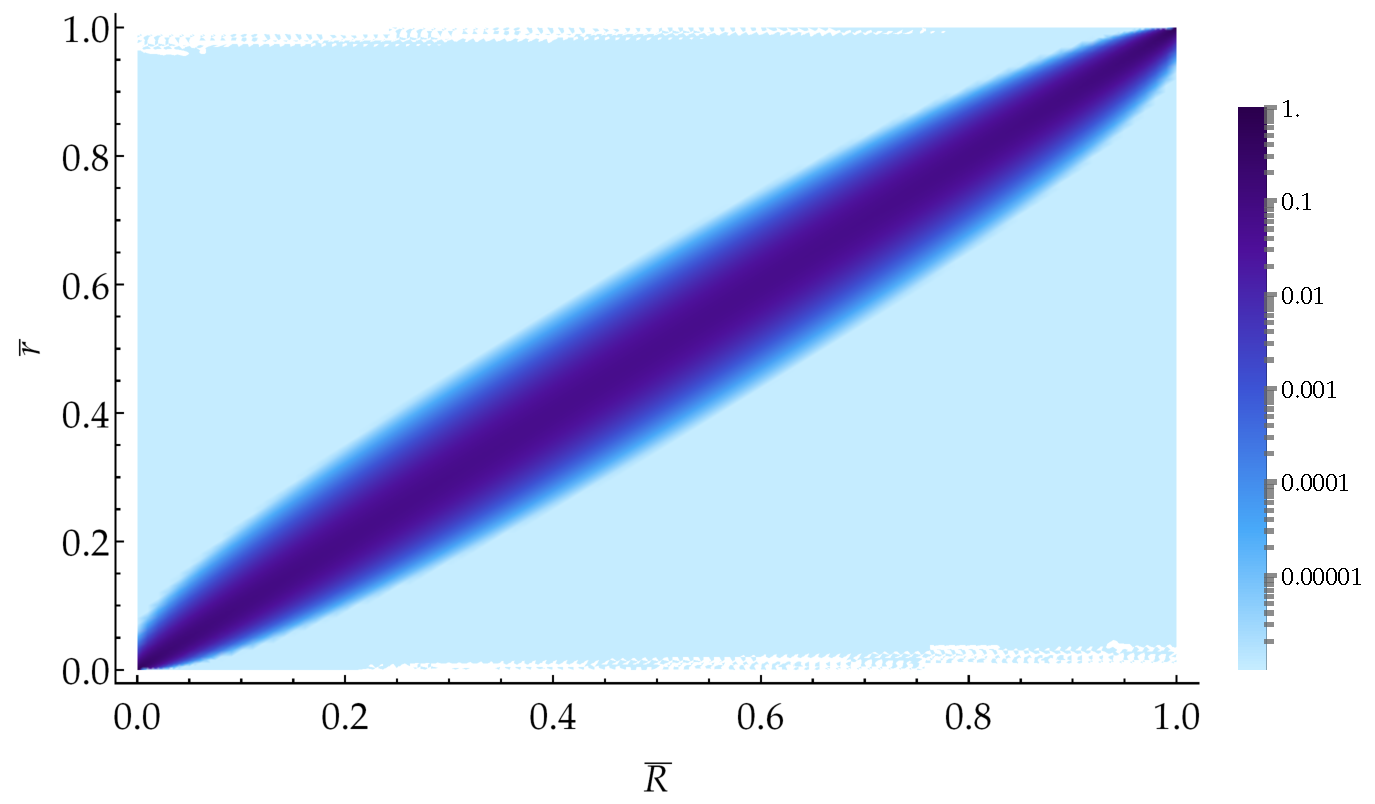
\includegraphics[width=\linewidth]{pop_sample_projection3.pdf}%
\caption{Log-density plot of the hypergeometric distribution
  $%\pf(\ya \|\yA, \yH)=
\yG_{\ya\yA} \defd  \raisebox{0pt}[0pt][1ex]{}\binom{n}{n\ya}\binom{N-n}{N \yA-n\ya}\binom{N}{N \yA}^{-1}$ for $N=5000$, $n=200$. (Band artifacts may appear in the
  colourbar depending on your \textsc{pdf} viewer.)}
\label{fig:hypergeom_proj}
\end{figure}%hypergeometric_identity.nb
These expectation equalities between sample and larger population should not
be surprising: we intuitively \emph{expect} that the proportion of coloured
balls sampled from an urn should be roughly equal to the proportion of
coloured ball contained in the urn. The formulae in the present section
formalize and mathematically express our intuition. The hypergeometric
distribution $\yG_{\ya\yA}$ plays an important role in this
formalization. A look at its plot, \fig~\ref{fig:hypergeom_proj}, reveals
that it is a sort of \enquote{fuzzy identity transformation}, or fuzzy
Kronecker delta, between the $\yA$-space $\set{0,\dotsc,N}$ and
$\ya$-space $\set{0,\dotsc,n}$. From \eqn~\eqref{eq:marginal} we thus have
that
\begin{equation}
  \label{eq:roughly_equal_nN}
  \pf(\ya=a \|\yH) \approx \pf(\yA=a \|\yH),\qquad
\E[\yg_{\ya} \|\yH] \approx \E[\yg_{\yA} \|\yH],
\end{equation}
where $\yg$ is any smooth function defined on $\clcl{0,1}$. These approximate
equalities express the intuitive fact that \emph{our uncertainty about the
  sample is representative of our uncertainty about the population and
  about other samples}, and vice versa. When $n=N$, $\yG_{\ya\yA}$
becomes the identity matrix and the approximate equalities above become
exact -- of course, since we have sampled the larger population.

But the approximate equalities above may miss important features of the two
probability distributions. In the next section we will in fact emphasize
their differences. If the distribution for the population average $\yA$ is
bimodal, for example, the bimodality can be lost in the distribution for
the sample average $\ya$, owing to the coarsening effect of
$\yG_{\ya\yA}$.

% They should be contrasted with the limits
% $\pf(\yxs=a) \to \pf(\yXf=a)$ and $\expeb{\yg_{\yxs}} \to \expeb{\yg_{\yXf}}$, as
% $n\to N$, do: these limits are trivially, universally valid because the
% sample becomes the larger population as $n\to N$. In particular, these limits
% hold even in cases where the conditional probability
% $\pf(\yxs = \ya \|\yXf=\yA)$ is not a fuzzy identity, our uncertainties
% about sample and about population can differ wildly, and the approximate
% equalities~\eqref{eq:roughly_equal_nN} do not hold.



\section{Maximum-entropy: sample level \vs\ larger-population level}
\label{sec:specific_initial_probability}

In the previous section we have seen that observations about a sample can
be used as constraints on the distribution for the activity of the larger
population. Let us use such constraints with the \me\ method. Suppose that
we want to constrain $m$ functions of the sample activity, vectorially
written $\yg \defd (c_1,\dotsc,c_m)$, to $m$ values
$\yc \defd (\widehat{c}_1,\dotsc,\widehat{c}_m)$. These functions are typically $k$-activities
$\sav{\yaa\dotso \yaa}$, and the values are typically the time averages of
the observed sample, as discussed in \sect~\ref{sec:intro}:
$\yc = \sum_t \yg[\ya(t)]/T$.

Let us apply the relative-\me\ method \citep{sivia1996_r2006,meadetal1984}
directly to sampled neurons; denote this approach by $\yHb$. Then we apply
the method to the larger population of neurons, most of which are unsampled;
denote this approach by $\yHa$.

Applied directly to the sampled neurons, the method yields the distribution
\begin{equation}
  \label{eq:app_maxent_sample}
  \pf(\ya \|\yHb)
  =\frac{1}{\yk(\yl)}\,
  \binom{n}{n\ya}
  \exp[\yl\T \yg_{\ya}]
\end{equation}
where $\yk(\yl)$ is a normalization constant. The binomial in front of the
exponential appears because we must account for the multiplicity by which
the population-average activity $\ya$ can be realized: $\ya=0$ can be
realized in only one way (all neurons inactive), $\ya=1/n$ can be realized
in $n$ ways (one active neuron out of $n$), and so on. This term is analogous to
the \enquote{density of states} in front of the Boltzmann factor in
statistical mechanics \citep[\chap~16]{callen1960_r1985}. The $m$ Lagrange
multipliers $\yl\defd (l_1,\dotsc,l_m)$ must satisfy the $m$ constraint
equations
\begin{equation}
  \label{eq:app_maxent_sample_constraints}
  \yc = \E(\yg \|\yHb) \equiv
  \frac{1}{\yk(\yl)}\sum_{\ya}  \yg_{\ya} \binom{n}{n\ya}
  \exp[\yl\T \yg_{\ya}].%, \qquad k=1,\dotsc,m.
\end{equation}

Applied to the larger population, using the constraint
expression~\eqref{eq:constraint_extended} derived in the previous section,
the method yields the distribution for the larger-population activity
\begin{equation}
  \label{eq:app_maxent_pop}
  \pf(\yA \| \yHa)  = \frac{1}{\yK(\yll)}\,
  \binom{N}{N \yA}\,\exp\bigl(\yll\T
  \tsum_{\ya} \yg_{\ya}\yG_{\ya\yA}\bigr).
\end{equation}
The $m$ Lagrange multipliers $\yll\defd (\lambda_1,\dotsc,\lambda_m)$ must
satisfy the $m$ constraint equations
\begin{equation}
  \label{eq:app_maxent_pop_constraints}
  \yc = \E(\yg \|\yHa)\equiv %{}\\
 \frac{1}{\yK(\yll)}\sum_{\ya} \sum_{\yA} \yg_{\ya} \yG_{\ya \yA}
\,
  \binom{N}{N \yA}\,\exp\bigl(\yll\T
  \tsum_{\ya} \yg_{\ya}\yG_{\ya\yA}\bigr).
%  \\ k=1,\dotsc,m.
\end{equation}

We obtain the distribution for the sample activity by marginalization, using
\eqn~\eqref{eq:marginal}:
\begin{equation}
  \label{eq:app_maxent_pop_marg}
  \pf(\ya \| \yHa)  = \frac{1}{\yK(\yll)}\, 
  \sum_{\yA} \yG_{\ya \yA}
\,
  \binom{N}{N \yA}\,\exp\bigl(\yll\T
  \tsum_{\ya} \yg_{\ya}\yG_{\ya\yA}\bigr).
\end{equation}

The distributions for the sample activity,
\eqns~\eqref{eq:app_maxent_pop_marg} and \eqref{eq:app_maxent_sample},
obtained with the two approaches $\yHb$ and $\yHa$, are different. From the
discussion in the previous section we expect them to be vaguely similar;
yet they cannot be exactly equal, because their equality would require the
$2m$ quantities $\yll$ and $\yl$ to satisfy the constraint equations
\eqref{eq:app_maxent_pop_constraints} and
\eqref{eq:app_maxent_sample_constraints}, and in addition also the $n$
equations $\pf(\ya \| \yHa) = \pf(\ya \| \yHb)$,
$\ya=1/n,\dotsc,1$ (one equation is taken care of by the normalization of
the distributions). We would have a set of $2m+n$ equations in $2m$
unknowns.

Hence, \emph{the applications of \me\ at the sample level and at the
  larger-population level are inequivalent}. They lead to numerically
different distributions for the sample activity $\yaa$.

%%% FIGURES %%%
\iffalse
\begin{figure}[!t]
\centering
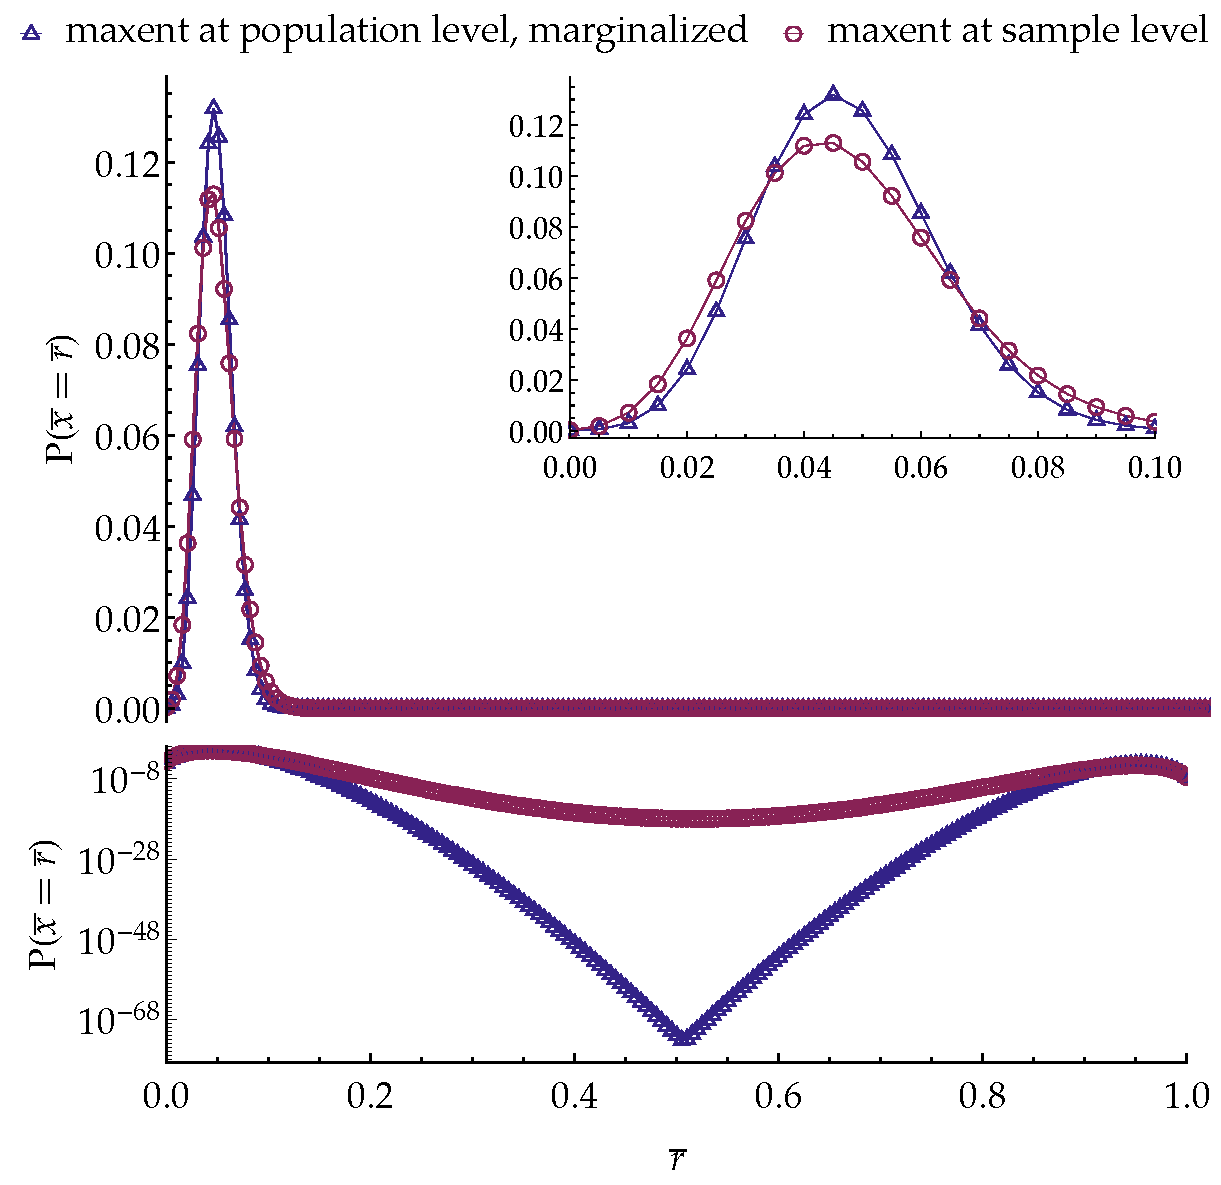
\includegraphics[width=\linewidth]{different_maxent_pop_sample_200_realdata_2mom.pdf}%
\caption{Linear and log-plots of $\pf(\ya)$ constructed by \me\ at
  the population level followed by sample marginalization (blue triangles),
  \eqn~\eqref{eq:app_maxent_pop_marg}, and at the sample level (red
  circles), \eqn~\eqref{eq:app_maxent_sample}, with $N=5000$,
  $n=200$, and constraints as in \eqn~\eqref{eq:constraints}.}
\label{fig:diff_maxent_pop_sample}
\end{figure}%maxent_pop_or_sample.nb
%
\begin{figure}[!t]
\centering
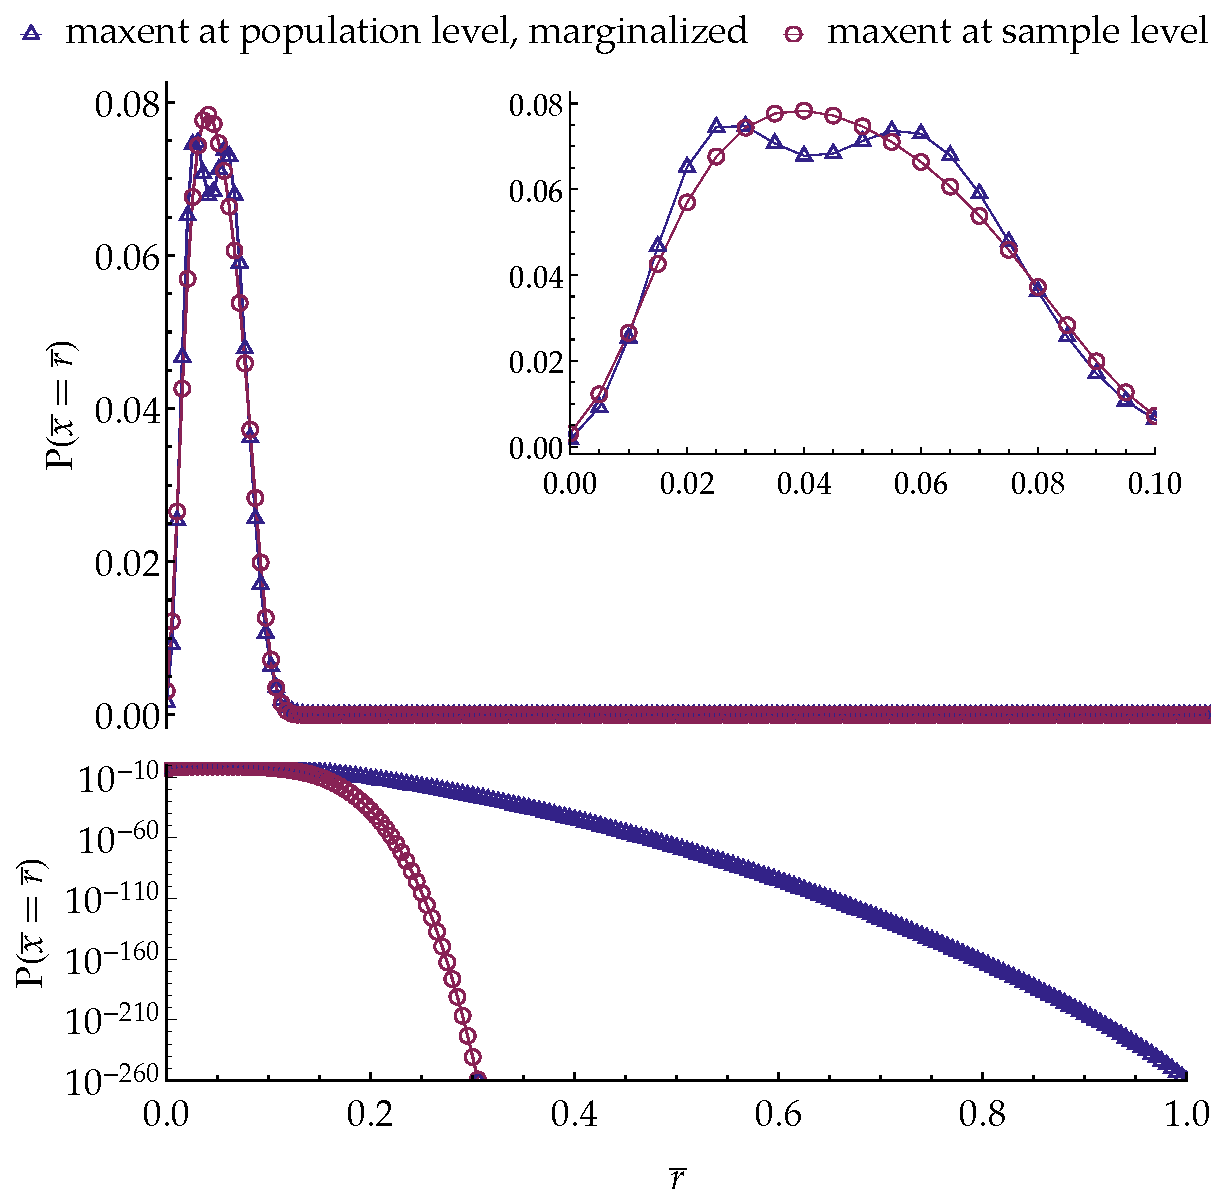
\includegraphics[width=\linewidth]{different_maxent_pop_sample_200_realdata_4mom.pdf}% 
\caption{Linear and log-plots of $\pf(\ya)$ constructed by \me\ at
  the population level followed by sample marginalization (blue triangles),
  \eqn~\eqref{eq:app_maxent_pop_marg}, and at the sample level (red
  circles), \eqn~\eqref{eq:app_maxent_sample}, with $N=5000$,
  $n=200$, and constraints as in \eqn~\eqref{eq:constraints}.}
\label{fig:diff_maxent_pop_sample_realdata}
\end{figure}%maxent_pop_or_sample.nb
\fi%
\begin{figure}[!t]
\centering
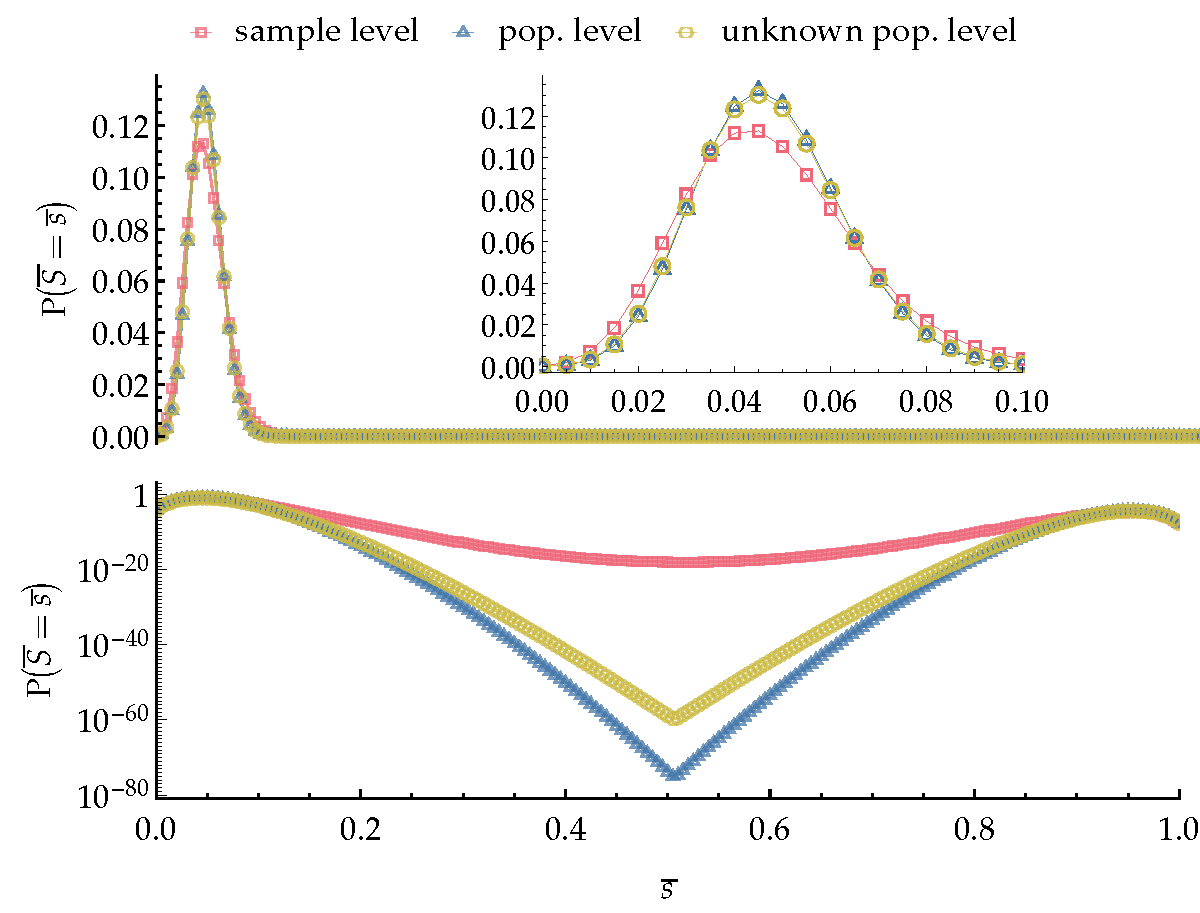
\includegraphics[width=\linewidth]{comparison3.pdf}%
\caption{Linear and log-plots of $\pf(\ya)$ for a sample of $n=200$
  and constraints as in \eqn~\eqref{eq:constraints}, constructed by:
  \textcolor{myred}{\textbf{red squares:}} \me\ at the sample level,
  \eqn~\eqref{eq:app_maxent_sample};
  \textcolor{mypurpleblue}{\textbf{blue triangles:}} \me\ at the
  population level, \eqn~\eqref{eq:app_maxent_pop_marg} with
  $N=10\,000$, followed by sample marginalization;
  \textcolor{myyellow}{\textbf{yellow circles:}} \me\ at the population
  level with unknown population size,
  \eqn~\eqref{eq:app_maxent_pop_marg_unknown_N}, according to the
  distribution~\eqref{eq:pdf_popsize} for the population.}
\label{fig:all_three}
\end{figure}%maxent_pop_or_sample.nb\fi
The distribution obtained at the sample level will show different
features from the one obtained at the population level, like displaced or
additional modes or particular tail behaviour. We show an example of this
discrepancy in \fig~\ref{fig:all_three}, for
$N=10\,000$, $n=200$, and the two constraints
\begin{equation}
  \label{eq:constraints}
  \E(\ya) = 0.0478,\qquad
  \E(\yaas) = 0.00257,
  % ,\quad
  % \expe{\sav{\yaa\yaa\yaa}} = 1.48\times 10^{-4},\quad
  % \expe{\sav{\yaa\yaa\yaa\yaa}} = 8.81 \times 10^{-6}.
\end{equation}
which come from the actual recording of circa 200 neurons from macaque
motor cortex \citep{rostamietal2016_r2017}. The distribution obtained at the
population level (blue triangles) has a higher and displaced mode and a quite
different behaviour for activities around $0.5$ than the distribution
obtained at the sample level (red squares).

\bigskip

In our discussion we have so far assumed the size $N$ of the larger
population to be known. This is rarely the case, however. We usually are
uncertain about $N$ and can only guess its order of magnitude. In such a
state of knowledge $\yHd$ our ignorance about the possible value of $N$
is expressed by a probability distribution $\pf(\yNN=N \|\yHd)=h(N)$,
and the marginal distribution for the sample
activity~\eqref{eq:app_maxent_pop_marg} is modified, by the law of total
probability, to
\begin{multline}
  \label{eq:app_maxent_pop_marg_unknown_N}
  \pf(\ya \| \yHd)  =
  \sum_{N} \pf(\ya \| N,\yHd) \,
  \pf(N \|\yHd)
  ={}\\[-\jot]
  \sum_N \biggl\{\frac{1}{\yK(\yll_N)}\, 
  \sum_{\yA} \yG^{(N)}_{\ya\yA}
\,
  \tbinom{N}{N \yA}\,\exp\Bigl[{\yll_N}\T
  \tsum_{\ya} \yg_{\ya}\yG^{(N)}_{\ya\yA}\Bigr]\biggr\}
  \;h(N),
\end{multline}
where the Lagrange multipliers $\yll_{N}$ and the summation range for
$\yA$ depend on $N$.

As a proof of concept, \fig~\ref{fig:all_three} also shows such a distribution
(yellow circles) for the same constraints as above, and a probability
distribution for $N$ inspired by Jeffreys
\citep[\sect~4.8]{jeffreys1939_r1983}:
\begin{equation}
  \label{eq:pdf_popsize}
  h(N) \propto 1/N, \qquad
  N \in\set{1\,000,\; 2\,000,\; \dotsc,\;10\,000}.
\end{equation}

\section{Derivation from the probability calculus}
\label{sec:derivation_prob_calculus}

There are three inequivalent main routes that lead to a probability
distribution of the maximum-entropy form~\eqref{eq:app_maxent_sample}
or~\eqref{eq:app_maxent_pop}. The distribution carries a different
interpretation under each route \citep[pp.~52--55,
72--77]{jaynes1979b}[pp.~25--28]{jaynes1982}[\sect~I]{jaynes1982b}{jaynes1986d_r1996}[\sect~11.1]{jaynes1994_r2003}.

\begin{enumerate}[wide,label=(\alph*)]
\item \label{item:entropy_route}One route is the choice of the distribution having the highest
  Shannon entropy, given only a quantitative assessment some of its
  properties, such as expectations. The numerical choice of the value of
  such properties is a (subjective) assumption.

  \medskip

  In the two other routes the maximum-entropy distribution is obtained as
  an \emph{approximation} of a distribution obtained via the probability
  calculus, using data coming from a set of $T$ measurements -- as in our
  present case.\mynote{refs here} Also in this case some (subjective)
  assumptions are necessary: they concern our beliefs about the long-run
  relative frequencies of the measurement outcomes:\footnote{Such
    assumptions are always necessary at the beginning of an inference:
    \enquote{Now the axioms of probability enable us to infer any
      probability-conclusion \emph{only} from probability-premisses. In
      other words, the calculus of probability does not enable us to infer
      any probability-value unless we have some probabilities or
      probability relations \emph{given}. Such data cannot be supplied by
      the mathematician. E.g. the rules of arithmetic and the axioms of the
      probability-calculus are utterly impotent to determine, on the
      supposed knowledge that the throw of a coin must yield either head or
      tail and cannot yield both, the probability that it will yield head
      or that it will yield tail. We must assume that the two co-exclusive
      and co-exhaustive possibilities are \emph{equally probable}, before
      we can estimate the probability of either as being a half of
      certitude} \citep[\emph{Appendix on eduction}, \sect~5,
    p.~182]{johnson1924}.}

\item \label{item:entr_prior_route}In one case we consider all possible
  sets of measurement outcomes to be \emph{roughly} equally likely; this
  leads to a probability for the frequencies $\ynu$ proportional to a
  multinomial coefficient $\binom{L}{L\ynu}$, with $L$ large but smaller
  than $T$. (We cannot assume the sets of measurement outcomes to be
  exactly equally likely, because this is equivalent to their independence:
  \cf\
  \cites[\sect~6.7]{jaynes1994_r2003}[\sect~B]{portamana2009}[\sect~2]{portamana2017}.)
  The exact expression is\mynote{equation here}
  %   \begin{multline}
  %   \label{eq:prob_conditional_average_exch}
  %   \p\bigl[\yE{N+1}{k} \bigcond \tsum\yo\yf{N}\in\yA, \yX\bigr] ={}\\
  %   \frac{\int\yqq_k\sum_{\yf{N}}  \delt(\tsum \yo\yf{N}\in \yA)\,
  %     \binom{N}{N\yf{N}}\,\bigl( \tprod \yq^{N\yf{N}} \bigr)  \,
  %     \pf(\yq \|\yX)  \,\di\yq}{ \int\sum_{\yf{N}} \delt(\tsum \yo\yf{N}\in \yA)\,
  %     \binom{N}{N\yf{N}}\,\bigl( \tprod \yq^{N\yf{N}} \bigr) \,
  %     \pf(\yq \|\yX) \,\di\yq },
  % \end{multline}

\item \label{item:suff_route}In the other case we assume that the
  measurements have a \emph{sufficient statistics}: the same as appears in
  the exponential of the maximum-entropy distribution. The exact expression is\mynote{equation here}
  % \begin{multline}
  %   \label{eq:prob_conditional_average_suff}
  %   \p\bigl[\yE{N+1}{k} \bigcond \tsum\yo\yf{N}\in\yA, \yS\bigr] ={}
  %       \\[3\jot]
  %    \frac{\int \pf(k \| \yl,\yaa,\yS) \sum_{\yf{N}} \delt(\tsum \yo\yf{N}\in \yA)\,
  %     \binom{N}{N\yf{N}}\,\bigl[ \tprod  \pf(\yk \| \yl,\yaa,\yS)^{N\yf{N}} \bigr]
  %      \,
  %     \pf(\yl \|\yS) \,\di\yl}{\int\sum_{\yf{N}} \delt(\tsum \yo\yf{N}\in \yA)\,
  %     \binom{N}{N\yf{N}}\,\bigl[ \tprod \pf(\yk \| \yl,\yaa,\yS)^{N\yf{N}} \bigr]
  %      \,
  %     \pf(\yl \|\yS) \,\di\yl}.
  % \end{multline}
\end{enumerate}

It's important to keep in mind that the approximate equivalence of these
three routes only holds under very specific assumptions -- which \emph{have
  physical and biological meanings and consequences}. In particular,
route~\ref{item:suff_route} implies that we can discard other empirical
statistics of the data, if they are known; whereas
route~\ref{item:entr_prior_route} requires us to specify all known
empirical statistics, because using only a subset of them may lead to
different results. Route~\ref{item:entropy_route} is also supposed to be
used with all known data. Moreover, the approximate equivalence of
route~\ref{item:entropy_route} with routes~\ref{item:entr_prior_route} and
\ref{item:suff_route} \emph{only holds if $T$ is much larger than the
  possible values of the activity $\yA$}. Finally, we also obtain very
different expressions depending on whether we're asking about \emph{the
  activity in one of the \textbf{recorded} time bins} or about \emph{the
  activity in a \textbf{new} time bin}. Works that use maximum-entropy
distributions are often very vague about the latter point.


\bigskip

Here are the distributions for our \dobs\ about three different quantities,
assuming an entropic pre-data distribution for the long-run frequencies of
the larger population:

\textbf{The frequency distribution $\yF$ of the larger-population activity
  \emph{during the recording}}

\begin{equation}
  \label{eq:fullfreq_from_samplefreq}
  \begin{split}
  \p(\yF \|\yf,\yH) &\propto
  \!\begin{multlined}[t][0.8\linewidth]
  \int\!\di\ynu\;  \tsum_{\yj}
  \delt(\tsum_{\yA}\yjj_{\ya\yA} = \yff_{\ya})\;
  \delt(\tsum_{\ya}\yjj_{\ya\yA} = \yFF_{\yA})\times{}\\
  \binom{T}{T\yj}\;
  \biggl[\prod_{\ya\yA}
(\yG_{\ya\yA}\ynuu_{\yA})^{T\yjj_{\ya\yA}}
\biggr]\;
\exp[-L\;\re(\ynu;\yR)]
\end{multlined}
\\
&\appropto \delt(\tsum_{\yA}\yG_{\ya\yA}\yFF_{\yA} = \yff_{\ya})\;
\exp[-L\;\re(\yF;\yR)]
\end{split}
\end{equation}

\bigskip

\textbf{The long-run frequency distribution $\ynu$ of the larger-population
  activity}

\begin{equation}
  \label{eq:longrun_from_samplefreq}
  \begin{split}
  \p(\ynu \|\yf,\yH) &\propto
    \binom{T}{T\yf}\;
  \biggl[\prod_{\ya}
(\tsum_{\yA}\yG_{\ya\yA}\ynuu_{\yA})^{T\yff_{\ya}}
\biggr]\;
\exp[-L\;\re(\ynu;\yR)]
\\
&\appropto 
\exp[-T\;\re(\yf; \mathte{\yG}\ynu)
-L\;\re(\ynu;\yR)]
\end{split}
\end{equation}
Note that if some $\yff_{\ya}$ are zero, then the first exponential may
be badly approximated by a delta, because the constraints lie on a facet of the
simplex of frequencies $\set{\ynu}$.

\bigskip

\textbf{The activity $\yA'$ of the larger-population
  in a \emph{new} time bin}

\begin{equation}
  \label{eq:newbin_from_samplefreq}
  \begin{split}
  \p(\yA' \|\yf,\yH) &\propto
  \int\!\di\ynu\;\ynuu_{\yA'}\;
  \binom{T}{T\yf}\;
  \biggl[\prod_{\ya}
(\tsum_{\yA}\yG_{\ya\yA}\ynuu_{\yA})^{T\yff_{\ya}}
\biggr]\;
\exp[-L\;\re(\ynu;\yR)]
\\
&\appropto 
\int\!\di\ynu\;\ynuu_{\yA'}\;
\exp[-T\;\re(\yf; \mathte{\yG}\ynu)
-L\;\re(\ynu;\yR)]
\end{split}
\end{equation}
Note that if some $\yff_{\ya}$ are zero, then the first exponential may
be badly approximated by a delta, because the constraints lie on a facet of the
simplex of frequencies $\set{\ynu}$.

\bigskip

The maximum-relative-entropy distribution is, in the first two cases, an
approximation of the most probable frequency distribution $\yF$ or $\ynu$;
in the third case, an approximation of the probability distribution for
$\yA'$.

\section{Assumptions and limitations}
\label{sec:assumptions}

Main assumptions behind this belief distribution:

We are approximating our state of knowledge with a finitely exchangeable
one. In turn, this is numerically approximated by an infinitely
exchangeable one for $T$ large. But we don't really have an exchangeable
belief: our \dob\ that the activity at the next time bin will
differ from the activity at the present one is roughly proportional to the
difference in the two subsequent activities.

The formulae say that we have equal beliefs about the underlying population
states having the same activity. This isn't really our belief, for we
believe there are interactions between the neurons and subpopulations thereof.


\section{Discussion}
\label{sec:discussion}

The purpose of the present work was to point out and show, in a simple
set-up, that the \me\ method can be applied to recorded neuronal data in a
way that accounts for the larger population from which the data are
sampled, \eqns~\eqref{eq:app_maxent_pop}--\eqref{eq:app_maxent_pop_marg}.
This application leads to results that differ from the standard application
which only considers the sample in isolation,
\eqns~\eqref{eq:app_maxent_sample}--\eqref{eq:app_maxent_sample_constraints}.
We gave a numerical example of this difference. We have also shown how to
extend the new application when the size of the larger population is
unknown, \eqn~\eqref{eq:app_maxent_pop_marg_unknown_N}.

The latter formula, in particular, shows that the standard way of applying
\me\ 
implicitly assumes that \emph{no} larger population exists beyond the
recorded sample of neurons. One could in fact object to the application at
the population level, and say that the traditional way of applying \me,
\eqn~\eqref{eq:app_maxent_sample}, yields different results because it does
not make assumptions about the size $N$ of a possibly existing larger
population. Such a state of uncertainty, however, is correctly formalized
according to the laws of probability by introducing a probability
distribution for $N$, and is expressed by
\eqn~\eqref{eq:app_maxent_pop_marg_unknown_N}. This expression cannot
generally be equal to~\eqref{eq:app_maxent_sample} unless the distribution
for $N$ gives unit probability to $N=n$; that is, unless the sample
\emph{is} the larger population, and no larger population exists.

The standard \me\ approach therefore assumes that the recorded neurons
constitute a special subpopulation, isolated from the larger population of
neurons in which it is embedded, and which was also present under the
recording device. This assumption is unrealistic. The \me\ approach at the
population level does not make such assumption and is therefore preferable.
It may reveal features in a data set that were unnoticed by the standard
\me\ approach.

% This hidden assumption of isolation is unreasonable. It amounts to say that
% the neurons we distinguished and tracked with our recording device are a
% very special, isolated set among all those that could have been recorded.
% It is for this reason that we find the \me\ application at the population
% level preferable. Physical models of neuronal populations usually include some
% sort of external input, mimicking an embedding in a larger population. The
% \me\ distribution obtained at the population level may reveal features in a
% data set that were unnoticed by the standard \me\ model.


The difference in the resulting distributions between the applications at
the sample and at the population levels appears in the use of Boltzmann
machines with hidden units \citep{lerouxetal2008}, although by a different
conceptual route. It also appears in statistical mechanics: if a system is
statistically described by a \me\ Gibbs state, its subsystems cannot be
described by a Gibbs state \citep{maesetal1999}. A somewhat similar
situation also appears in the statistical description of the final state of
a non-equilibrium process starting and ending in two equilibrium states: we
can describe our knowledge about the final state either by (1) a Gibbs
distribution, calculated from the final equilibrium macrovariables, or (2)
by the distribution obtained from the Liouville evolution of the Gibbs
distribution assigned to the initial state. The two distributions differ
(even though the final \emph{physical} state is obviously exactly the same
\citep[\sect~4]{jaynes1985d_r1993}), and the second allows us to make
sharper predictions about the final physical state thanks to our knowledge
of its preceding dynamics. In this example, though, both distributions are
usually extremely sharp and practically lead to the same predictions. In
neuroscientific applications, the difference in predictions of the sample
\vs\ larger-population applications can instead be very relevant.

The idea of the new application leads in fact to more questions. For
instance:
\begin{itemize}
\item Do the standard and new applications lead to different or contrasting
  conclusions about \enquote{cooperativity}, when applied to real data
  sets?
\item How to extend the new application to the \enquote{inhomogeneous} case
  \citep{schneidmanetal2006,shlensetal2006,roudietal2009b}, in which
  expectations for individual neurons or groups of neurons are constrained?
\item What is the mathematical relation between the new application and
  \me\ models with hidden neurons
  \citep{smolensky1986,kulkarnietal2007,huang2015,dunnetal2017}?
\end{itemize}
Owing to space limitations we must leave a thorough investigation of these
questions to future work.

Finally, we would like to point out the usefulness and importance of the
probability formulae that relate our states of knowledge about a population
and its samples, presented in \sect~\ref{sec:prob_samples}. This kind of
formulae is essential in neuroscience, where we try to understand
properties of extended brain areas from partial observations. The
formulae presented here reflect a simple, symmetric state of ignorance.
More work is needed \citep[\cf][]{levinaetal2017} to extend these formulae
to account for finer knowledge of the cerebral cortex and its population
properties.


\clearpage

\hrule
\newcounter{dummy}\refstepcounter{dummy}\label{orig_intro}
\mynote{orig intro}
Experimental technologies to record the activity of many neurons at the
same time in different species and brain areas are rapidly advancing. These
experimental advancements are paralleled by advances in theoretical and
computational methods for analyzing the data accumulated using the
recording technologies. Such theoretical methods usually take the form of
probabilistic models that try to describe the multi-neuronal activity of
the recorded neurons. With such probabilistic models one aims to address
numerous issues: What correlations are important in describing the
multi-neuronal pattern? How does the pattern of activity covary with
external stimuli or experimental conditions? What dimensionality does the
neural data live in and how is this related to the underlying population
interactions? The probabilistic models can also be used to make predictions
about the structure of the neural code, by studying the properties of the
fitted model, or by generating synthetic data from it.

In general, despite the rapid advances in recording technology, the best
experimental measurements of neuronal activity still only provide data from
a small subset of neurons that comprise a neuronal population. A wealth of
studies on building probabilistic models of neural data focuses on
describing such subsets, ignoring the fact that the observed neurons is a
small group in a much bigger set of hidden neurons. Some other studies do
include hidden variables which, amongst other things, aim to model the
global features of the unrecorded neurons, but we still lack a through
understanding of how to include the role of hidden neurons in probabilistic
models, how our inferences about the recorded activity would be affected by
them, and what we can we say about the rest of the population by studying the
heavily subsampled recordings. In this paper, we aim to address these
questions in the case of a simple maximum entropy model, namely the
homogeneous maximum entropy model.

The maximum entropy approach has been used in a variety of setting for
building statistical models of complex systems and datasets, ranging from
neuronal activity in the retina, in the cortex, protein sequences, gene
regulatory populations and natural images. The general idea is, for a dataset,
to write down the distribution that maximizes the entropy of state
variables, given some low order statistics. Now given the fact that the
recorded neurons are a fraction of the neurons in the population, several
quantitative questions arise that we will address in this paper: given the
data from the sampled neurons, can we build a maximum entropy model over
the whole population? Once we build such a population level maximum entropy
model, can we see features in the neural activity which cannot be directly
seen from a model build from the sampled neurons? Since we can marginalize
down the population level maximum entropy model to the sampled population, how
does this margianzlied maximum entropy model match the sample level model?

All these questions can be answered in the case of the homogeneous maximum
entropy model. First we show how to go from the sample level maximum
entropy level to the population level, by assuming different sizes of the
population and also by assuming an uninformative prior over the size of the
population. This is done by inferring the statistics of correlation functions
at the population level from those of the sample level by using simple
counting arguments. We then find that, when applied to experimental
recordings from the Medial Entorhinal Cortex of rats and the monkey visual
cortex, this population level maximum entropy model may exhibit features that
the sample level model does not predict. Specifically, we observed modes in
the distribution of the activity in the population level model that do not
show up in the sample level. We study how the assumed size of the larger
population affects the appearance of these modes and find that there is a
minimum size of the larger population for which such modes can be observed. We
then compared the distribution found by marginalizing the larger population
maximum entropy model down to the sample level, and the distribution fit
directly to the sample level. For the two datasets that we tested, we found
that the two distributions match each other to a large degree but that
there are also differences between them. We quantify how these differences
also depend on the assumed size of the population and find that …(WE SHOULD
TEST SHI) This predicts that for a large enough population (DO WE PREDICT
THAT IF THE LARGER POPULATION GETS BIGGER THE DIFFERENCE ALSO GET BIGGER)?…

The rest of the paper is organized as follows. We first describe how to go
from the sample level maximum entropy model to the larger population maximum
entropy model. In section 2, we apply this to the two experimental datasets
and study the effect of the assumed size of the population as well as the
moments that we use for building the maximum entropy model. In section 3 we
compare the distributions found from marginalizing the maximum entropy
model down to the sample level and the original sample level model.


\hrule
\bigskip

%%% Local Variables: 
%%% mode: LaTeX
%%% TeX-PDF-mode: t
%%% TeX-master: t
%%% End: 
